% Template Acknowledgements:
%% bare_jrnl.tex
%% V1.4b
%% 2015/08/26
%% by Michael Shell
%% see http://www.michaelshell.org/
%% for current contact information.
\documentclass[journal]{IEEEtran}
\usepackage{hyperref}
\usepackage[pdftex]{graphicx}
\usepackage{textcomp}
\graphicspath{{../figures/}}

\begin{document}

\title{Colorimetric Detection of pH Strips}
\author{Aman~Dhar,~
        Rudra~Mehta,~
        and~Matthew~Sit
\thanks{The project is to create and test various machine learning models to conclude upon the best way to find the pH of a biochemical solution, given an image of a pH test strip that has been applied to that solution.

All three of the authors are undergraduates completing this project for extra credit for CS 189 at UC Berkeley in Fall 2017. Rudra and Matthew submitted a more applied view on this topic for their final project for BioE 134, Genetic Design Automation, in which they trained and hyperparameter tuned a variety of models in order to accomplish the task practically. Here for CS 189, we replicate, comment on, and critique Mutlu, et al., 2017, which approaches this task using Support Vector Machines. Some background research, data collection, and fundamental modeling approaches may overlap, but the written deliverables and area of analyses will be unique. Permission to submit a related project to CS 189 has been provided by the BioE 134 professor, John Christopher Anderson (jcanderson@berkeley.edu).

All of our source code is available at \url{https://github.com/mattsit/ph-machine-learning.}}}

% The paper headers
\markboth{EECS 189,~University of California, Berkeley, December~2017}%
{Shell \MakeLowercase{\textit{et al.}}: Bare Demo of IEEEtran.cls for IEEE Journals}

% make the title area
\maketitle

\begin{abstract}
In this paper, we apply several machine learning techniques and models for the purpose of classifying and estimating the pH of solutions given raw image data of pH test strips. We replicate and critique much of the work performed by Mutlu et. al \cite{mutlu}, who used LS-SVM and claimed to achieve 100\% classification. We believe that this high accuracy was the result of duplicating physical pH strips samples between training and validation datasets; this is problematic because the noise between different strips of the same class was not accounted for, and samples were essentially duplicated as pre-processing mitigated orientation variability efforts. We further find that regression is a more suitable approach for this domain, as pH values are on a continuous, logarithmic scale, and decimal differences in value can have significant biological consequences. In this spirit, we find that mean squared regression errors as low as $\sim$0.033 are achievable.
\end{abstract}

\begin{IEEEkeywords}
machine learning, regression, classification, support vector machine, linear discriminant analysis, nearest neighbors, pH, principal component analysis, image processing.
\end{IEEEkeywords}

\IEEEpeerreviewmaketitle

\section{Introduction}
\IEEEPARstart{G}{rowing} cell cultures for industrial-scale chemical output is a very difficult task. Large bioreactors cost tens of thousands of dollars and require complex, specialized machinery to operate. An alternative idea is to make use of many 5-gallon buckets, with a Tyvek membrane on top that allows air to pass through the system, but blocks liquids \cite{anderson}. With a pump inside the bucket to mix nutrients with the cells, we essentially have a low-cost bioreactor. We need to test the pH of each bucket periodically to determine when to feed the cells. This can be done in a cost-effective manner by using paper-based strips that are briefly submerged into the solution. This method of bioreactors can only be profitable if there are many buckets - on the order of hundreds or thousands. Therefore, we need an efficient, automated method of determining pH from the test strips. The literature on this suggest that in practice, smartphones are used as the source of these pictures \cite{mutlu}, \cite{kim}.

Mutlu, et al., 2017, uses a Least Squares Support Vector Machine and a Support Vector Machine in order to classify images of pH strips by their pH values, capturing the images using a Smartphone camera and with various lighting and positional arrangement conditions \cite{mutlu}.

In this paper, we critique Mutlu, et al. by discussing the experimental design choices made, replicating the experimental conditions tested to the best we can under our limitations, and extending their work to regression, which we argue is more scientifically relevant and has higher utility.

\section{Experimental Setup and Pre-Processing}

\begin{figure}
\centering
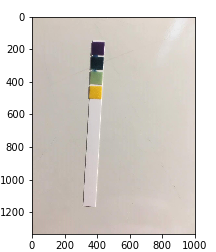
\includegraphics[height=2in]{raw8p70_07.png}
\caption{A photo of a pH strip captured with a hand-held smartphone under standard household lighting. This pH strip was submersed in a buffer with a target pH value of 8.70. The wet pH strip occasionally had solution leak across panels.}
\label{raw_photo}
\end{figure}

We collected our own data for this study. Mutlu was able to capture the range of pH values comprehensively through the use of adjustable chemical buffers. This allowed them to train on chemical solutions with integer pH values. They also were able to determine ground-truth labels for their data points by using a digitized pH meter. We were more limited in our resources; we had a fixed set of non-adjustable buffers and we took the label on the bottle as the ground-truth label for regression. In total we hand-held a smartphone to capture 10 samples under standard household lighting of pH strips submersed in the following 9 buffers: 2.22, 4.40, 4.47, 5.31, 6.28, 7.00, 7.70, 8.70, 10.0 (Fig. \ref{raw_photo}). These fixed non-integer pH values may be a source of irreducible error for us when we rounded these values to the nearest integer when performing classification. However, we wanted our model to be more robust to noise and to be applicable in a more reasonable environment, where a researcher would not have to use a custom apparatus remove any external sources of light \cite{mutlu}, \cite{kim}. Mutlu waited for the strips to dry before taking pictures, but we decided to capture the images while they were still wet since we imagine that pH strips are read while wet in practice.

We note that for each sample taken, we submersed a fresh pH strip into the solution, which is in contrast to the procedure Mutlu used. This approach is better because when Mutlu took multiple pictures of the same physical strip, they introduced any peculiarities of that strip into the dataset multiple times. Even though Mutlu exposed that physical strip to different lighting conditions and orientations before taking its picture again, any noisy details unique to that strip remained in all photos taken of it. We also argue that after their pre-processing techniques of specific orientation rotations and gamma corrections, many of these images may have ended up extremely similar regardless. Also, due to the symmetric nature of a camera flash, many of their rotations will receive the same lighting conditions from the flash, thus compounding the issue of reusing data. This can potentially lead to a false inflation in model accuracy due to images of the same physical strip being in both the training and testing set during k-fold cross-validation.

Mutlu performed experiments in which images were captured under various lighting conditions: with a light-shielding apparatus, without the apparatus, sunlight, fluorescent, and halogen. The intent of this was to show that a model trained under one lighting condition could be used to predict samples from another condition with reasonable accuracy. In the pre-processing stage, Mutlu rotates the images so that the strips are all in the same orientation. We do not do this because all of our photos were taken with the strip in a relatively vertical position. In fact, we argue that Mutlu’s efforts to arrange the pH strips in random positions and orientations is removed by their pre-processing efforts before this feature is exposed to the model. Mutlu also saves the images under a variety of filetype formats to see if there is any effect. We did not do this since they did not report any significant differences and this may be because this is similar to downsampling since the fidelity of the image data is never significantly compromised. Further, Mutlu performs gamma-correction during pre-processing. We argue that this should not be done since this relies upon prior information on how the given lighting condition is to be handled; Mutlu reports that when lighting conditions were mixed, accuracy decreased and we believe that this is because gamma-correction at pre-processing was not as effective. At the conclusion of pre-processing, Mutlu extracts out the RGB color values for each of the four panels of the pH strip to use as 12 features for the models.

\begin{figure}
\centering
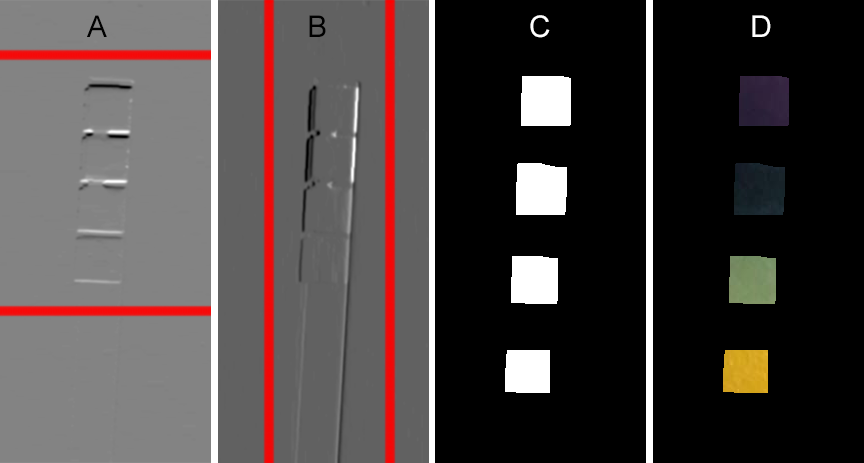
\includegraphics[width=3.25in]{Fig_2.png}
\caption{Image preprocessing procedure: (A) Horizontal Sobel filter applied on a grayscaled pH strip image. The red lines represent the regions to crop the image at. (B) Vertical Sobel filter applied on a grayscaled pH strip image. The red lines represent the regions to crop the image at. (C) Binarized mask of the original image, cropped based on the Sobel filters, and eroded to get the center color regions. (D) Final masked image, isolating the four color squares.}
\label{pre-process}
\end{figure}

For our study, as Mutlu did, we extract out the RBG values from the four panels, but we do this as our first step and use these original features for our first experiment. In order to extract the colors, we first crop the original image using the box specified from the horizontal (Fig. \ref{pre-process}a) and vertical (Fig. \ref{pre-process}b) Sobel edge-detection filters, as illustrated by the red lines in the images. We then apply a repeatedly-opened, distance eroded binary threshold (Fig. \ref{pre-process}c) to get the center regions of each color square from the original image (Fig. \ref{pre-process}d).

\begin{figure}
\centering
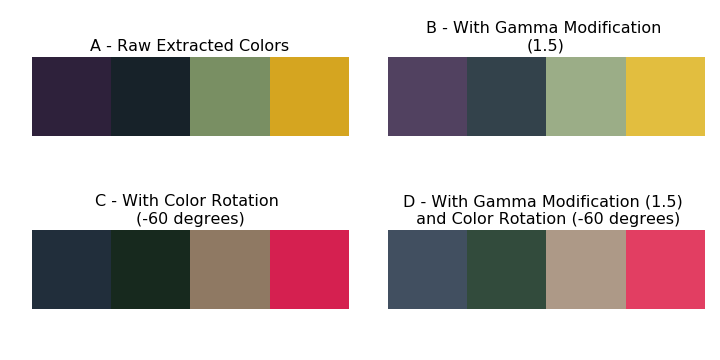
\includegraphics[width=3.25in]{Fig_3.png}
\caption{(A) The colors extracted from the four panels of a pH strip, stored in code as a total of 12 RGB values. (B) Gamma correction with a parameter of 1.5 applied on the raw extracted colors. Gamma correction nonlinear maps each color to effectively lighten or darken the image. (C) Hue rotation of -60 degrees around the color wheel applied on the raw extracted colors. (D) Application of both a gamma correction of 1.5 and a hue rotation of -60 degrees on the raw extracted colors.}
\label{four-colors}
\end{figure}

From there, we extract the 12 features by taking the average value RBG values from each of the four color boxes (Fig. \ref{four-colors}a). We then generalize Mutlu’s experiments by artificially applying randomly generated lighting conditions to our data. This way, we do not correct for lighting before training a model like Mutlu does but rather, introduce lighting conditions to our homogeneous dataset so that our model can learn to ignore lighting conditions on its own, rather than having to rely on manual and lighting condition-specific pre-processing methods. Specifically, in our second experiment, we gamma correct each sample with a uniformly chosen coefficient between 0.5 and 1.5 (Fig. \ref{four-colors}b) because this mimics the nonlinear luminescence introduced in captured images \cite{farid}. In our third experiment, we perform hue rotation with a uniformly chosen degree between -90 and 90 degrees (Fig. \ref{four-colors}c). In our fourth experiment, we apply the random lighting conditions from both experiments 2 and 3 simultaneously (Fig. \ref{four-colors}d).

Both Mutlu and we round our pH labels to the nearest integer and use one-hot encoding to represent the 15 pH value classes (from 0 to 14). We both also divided our data into training and validation sets in a k-fold cross validation fashion. Mutlu used k=10 according to the literature, while we chose k=3 in a stratified fashion in order to guarantee that samples from each class are present in all our training and validation sets (since we only had 90 data points to work with).

While Mutlu tested support vector machines (SVM) and least-squares support vector machines (LS-SVM) models for classification, we chose to use a much wider suite of both regression and classification models, including ridge regression, linear discriminant analysis (LDA), SVM, and k-nearest neighbors (kNN) in an effort to achieve higher test set accuracy. We also performed grid searches over several hyperparameters for each model, and employed scaling and dimensionality reduction techniques like principal component analysis (PCA) to further boost accuracy for certain methods.

For our study, we used Python 3.6.3, NumPy 1.13.3, scikit-learn 0.19.1, Matplotlib 2.1.0, and Open Source Computer Vision Library 3.3.0.

\section{Results}

\subsection{Pre-Processing}
\begin{figure}
\centering
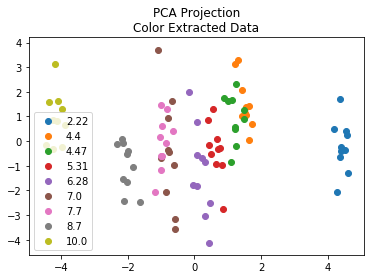
\includegraphics[height=2.5in]{pca.png}
\caption{Raw color extracted data projected onto two orthogonal axes such that variance captured is maximized.}
\label{pca}
\end{figure}

For select experiments, we used PCA in order to project our data into a lower-dimensional subspace in order to simplify our models and hopefully increase accuracy. We hyperparameter tuned across different numbers of components for the applicable models. We can see that the classes cluster well, even with projection onto only two axes (Fig. \ref{pca}).

\subsection{Classification Models}

\begin{figure}
\centering
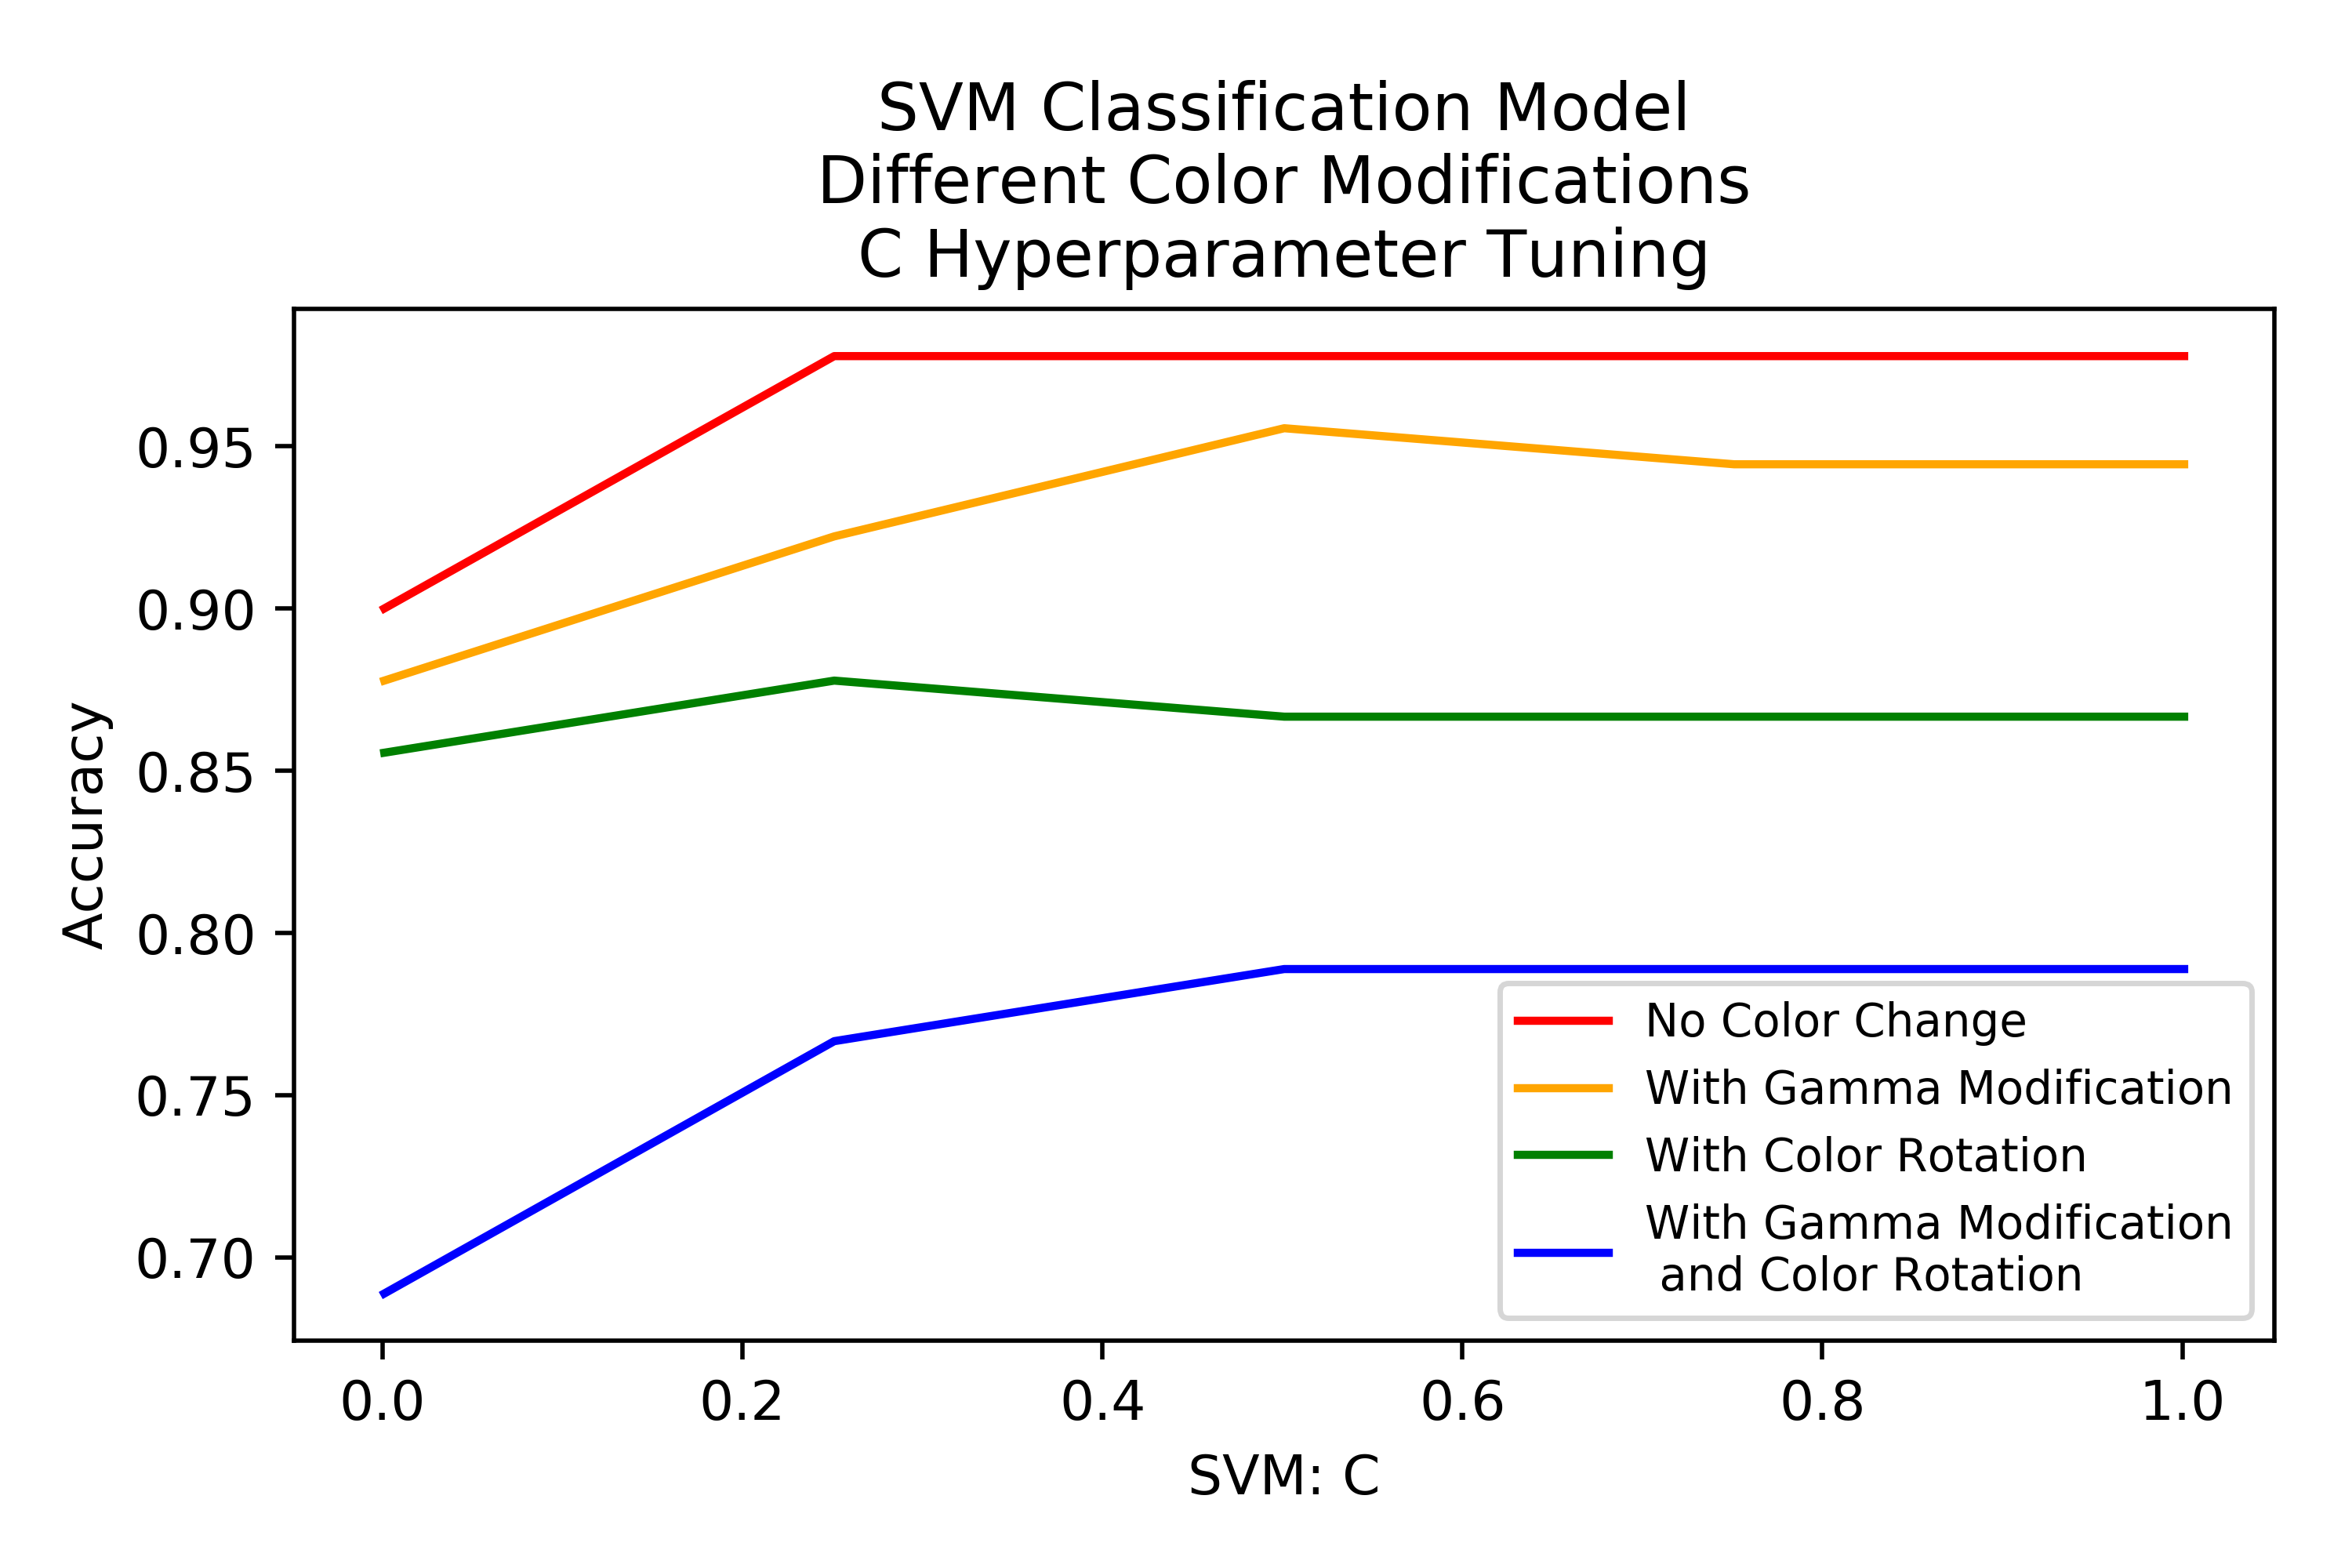
\includegraphics[height=2in]{SVM/svm_classification.png}
\caption{Support Vector Machine Classification Model. The Y axis is the Accuracy (percent of predicted labels that are correct) and the X axis is the regularization strength. The four lines represent the four datasets we used: no color change, with gamma modification, with color rotation, and with both gamma modification and color rotation.}
\label{svm}

\centering
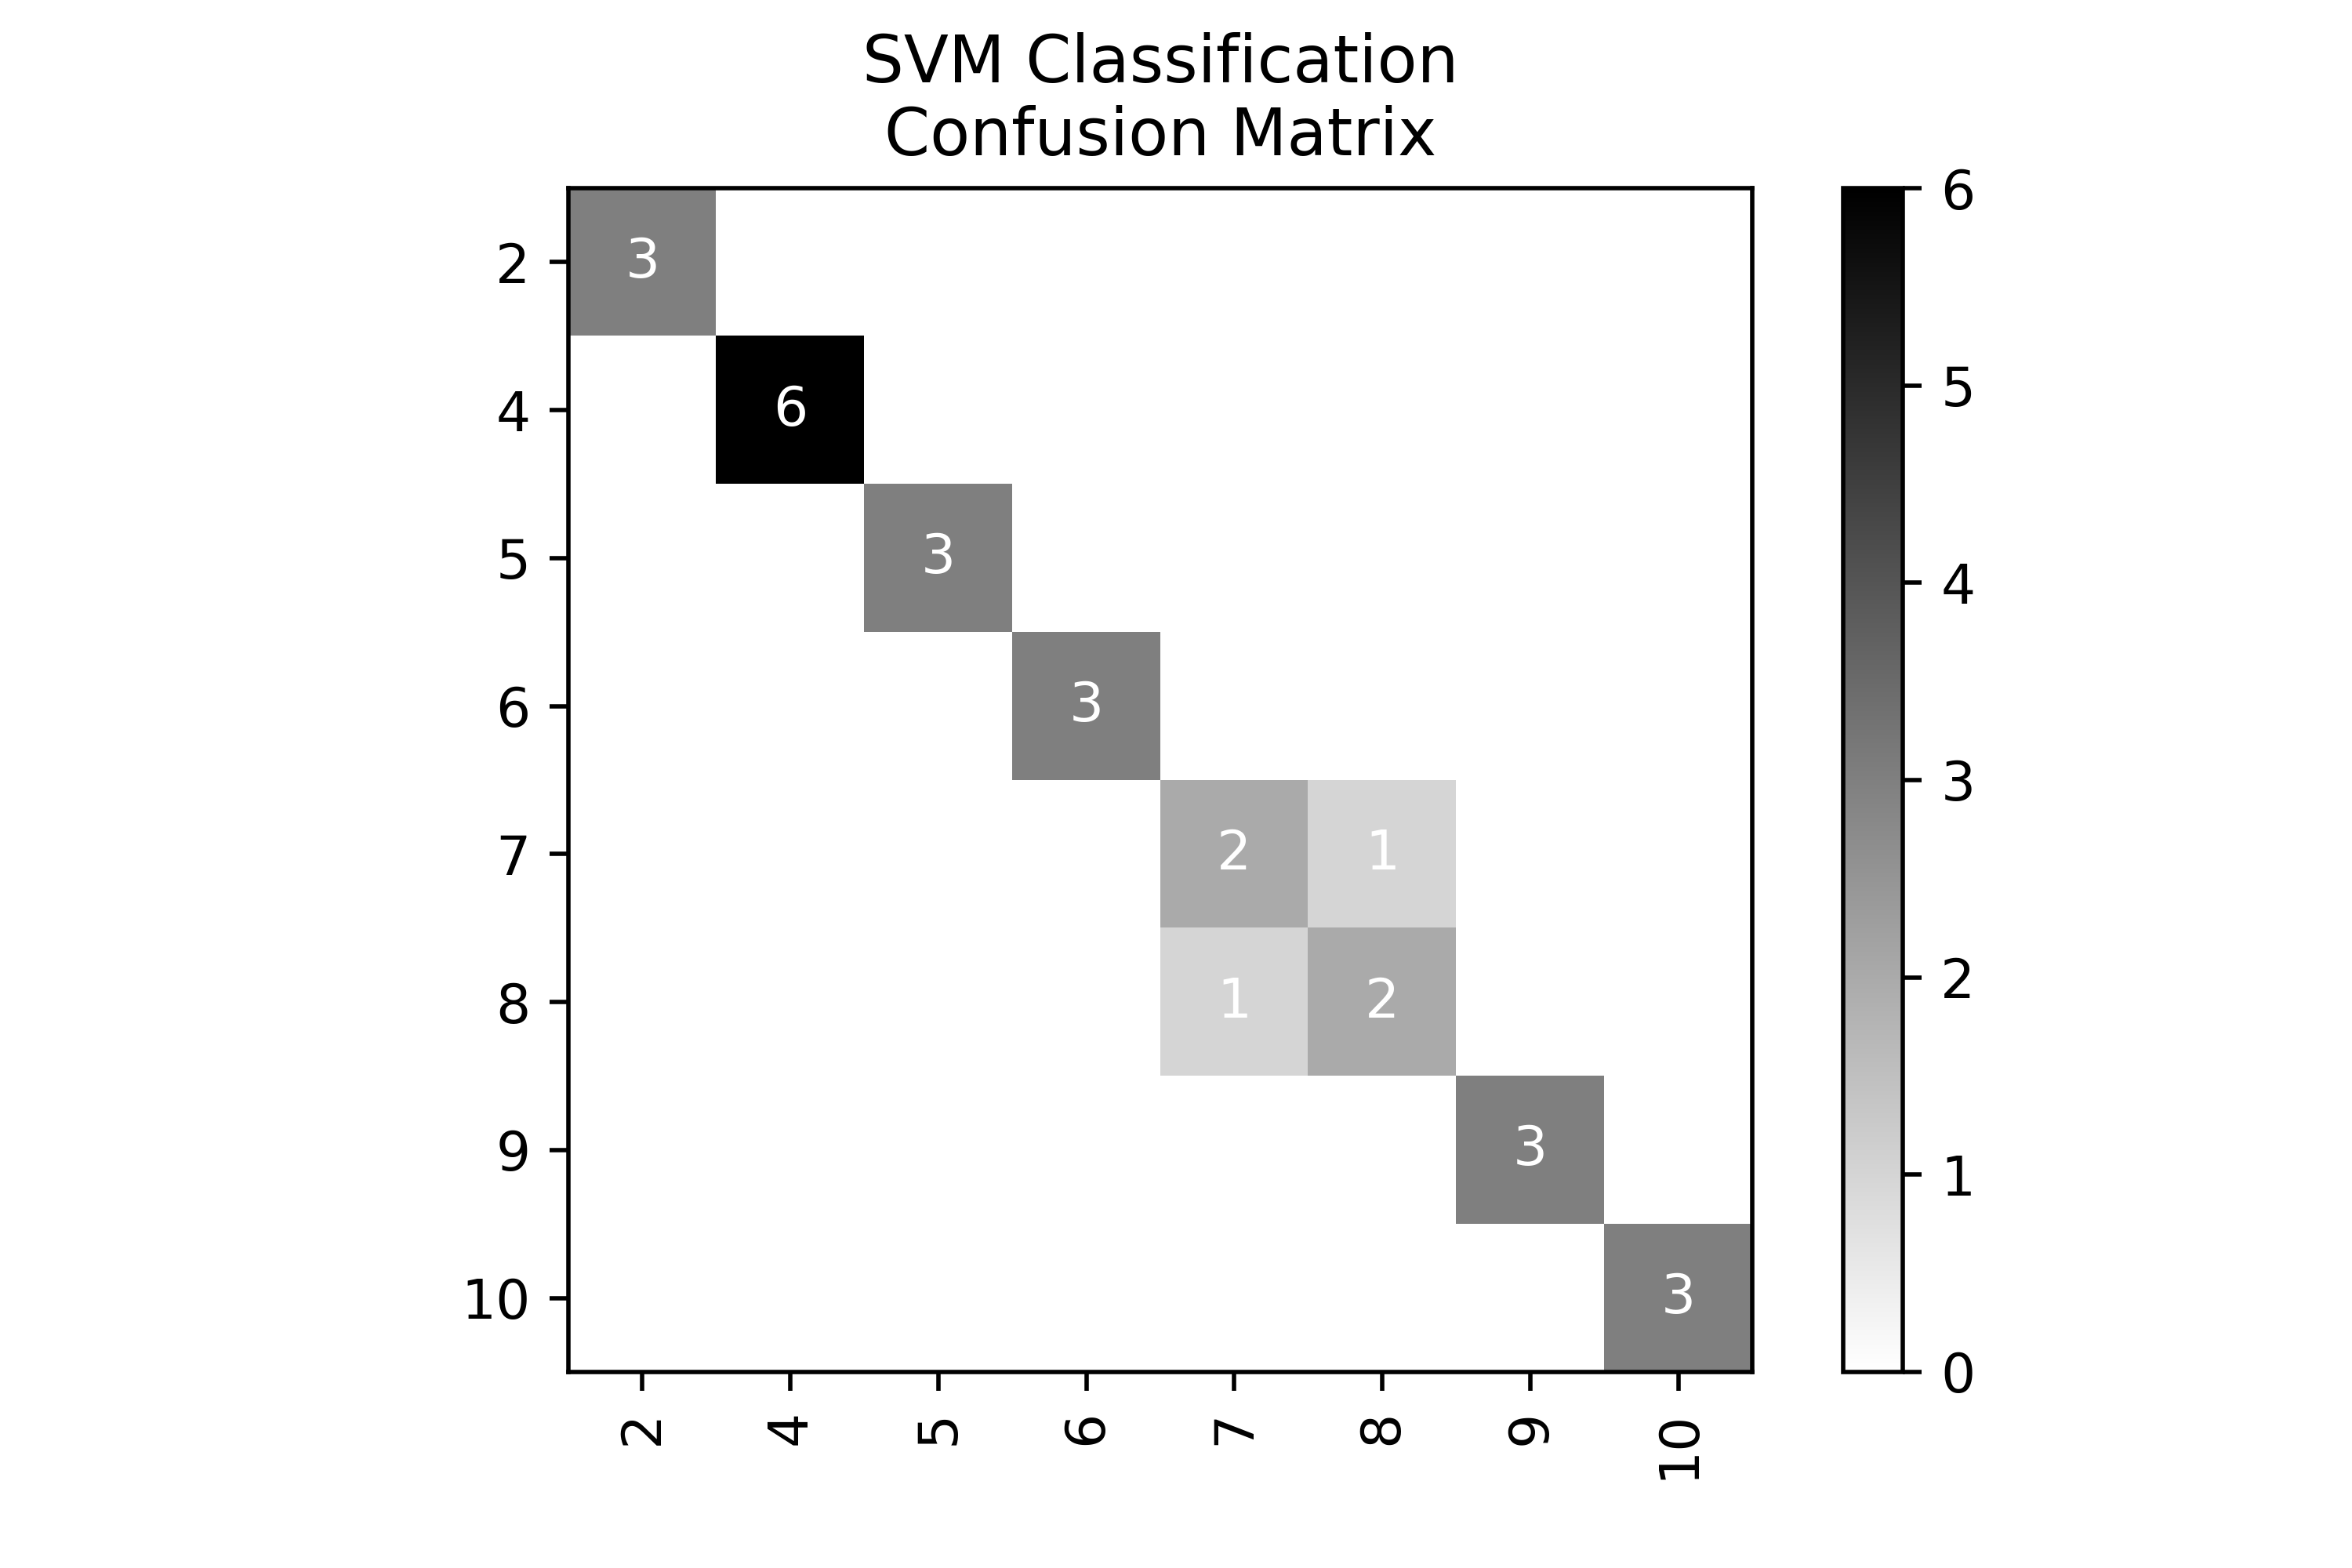
\includegraphics[height=2.5in]{SVM/SVM_classification_cfm.png}
\caption{Sample confusion matrix for one fold of three-fold cross validation for SVM model. The confusion matrix plots the predicted class on the X axis, and the true class on the Y axis. Therefore, elements along the diagonal of the matrix were predicted correctly. In this case, 2 of 27 images were misclassified.}
\label{svm_confusion}
\end{figure}

As in the Mutlu paper, we first used Support Vector Machines (SVM) for classification across the four experiments. Classification accuracies of $98\%$, $96\%$, $88\%$, and $79\%$ were achieved using 7, 8, 9, and 9 PCA-derived components respectively. As the regularization strength decreased, the accuracies for all but the third experiment generally increased. The third experiment’s SVM model performed slightly better with greater regularization strength (Fig. \ref{svm}, \ref{svm_confusion}).

\begin{figure}
\centering
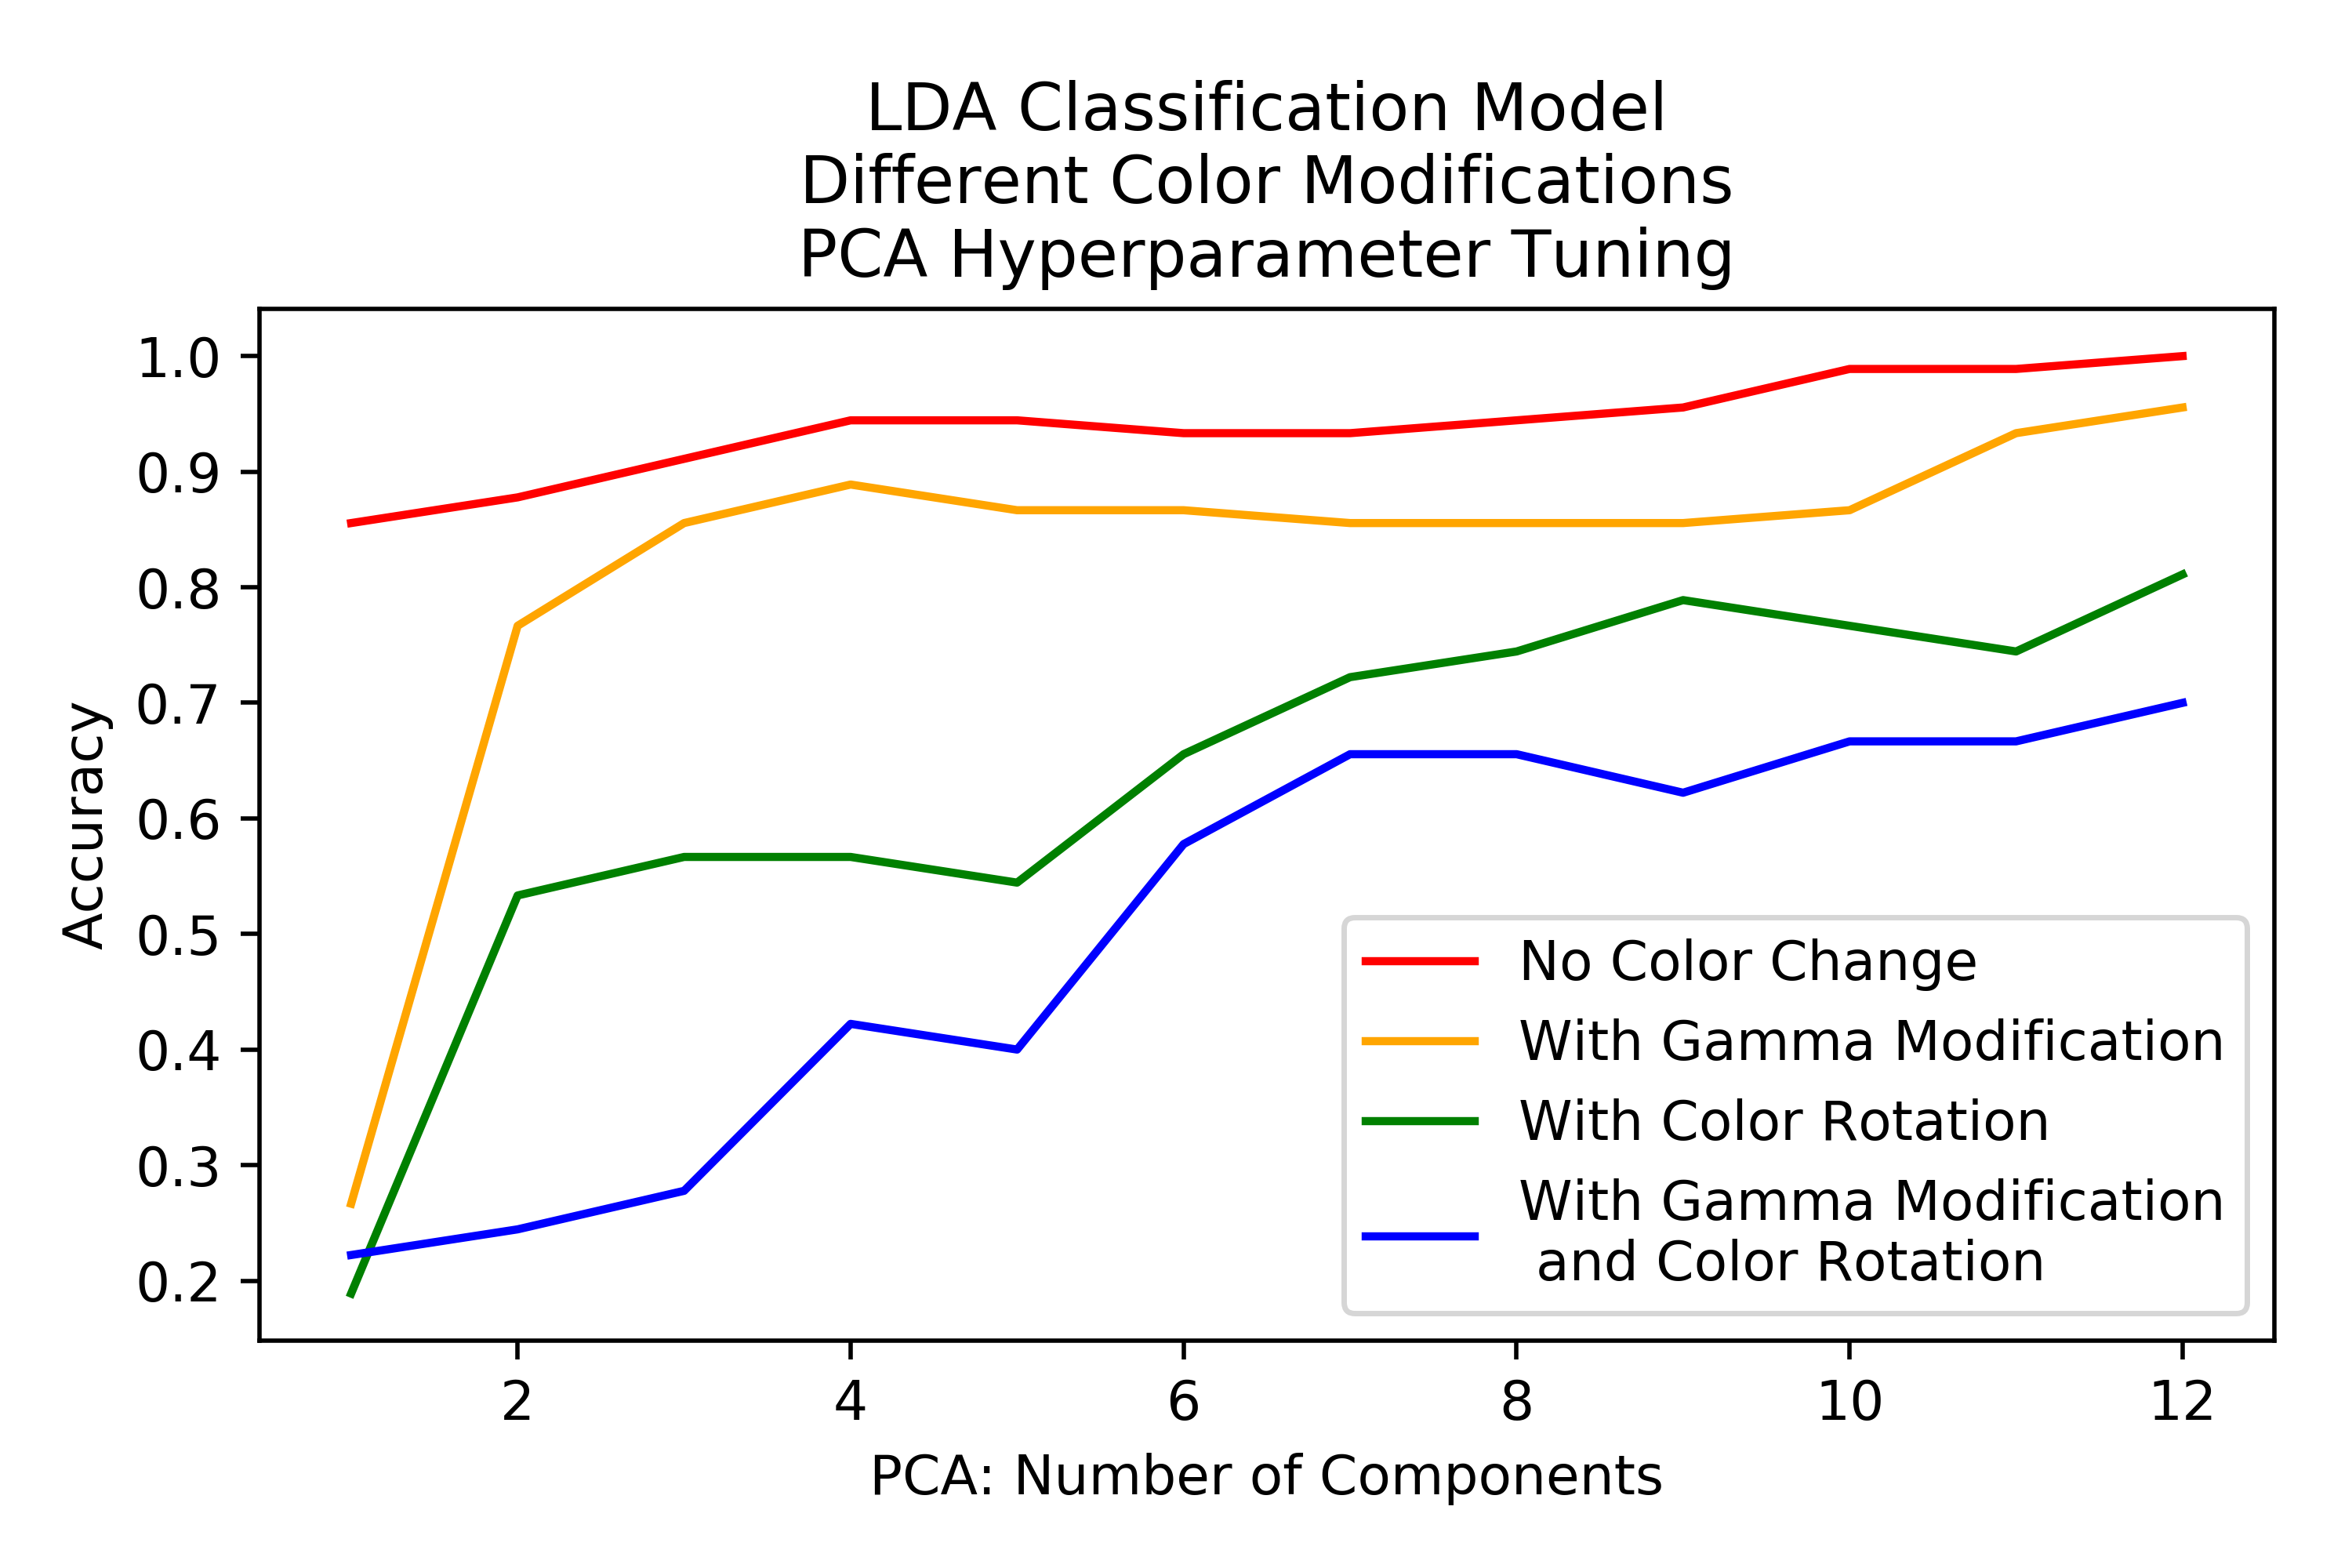
\includegraphics[height=2in]{LDA/lda_classification.png}
\caption{Linear Discriminant Analysis Classification Model. The Y axis is the Accuracy (percent of predicted labels that are correct) and the X axis is different number of components we project the data onto when doing PCA. The four lines represent the four datasets we used: no color change, with gamma modification, with color rotation, and with both gamma modification and color rotation.}
\label{lda}

\centering
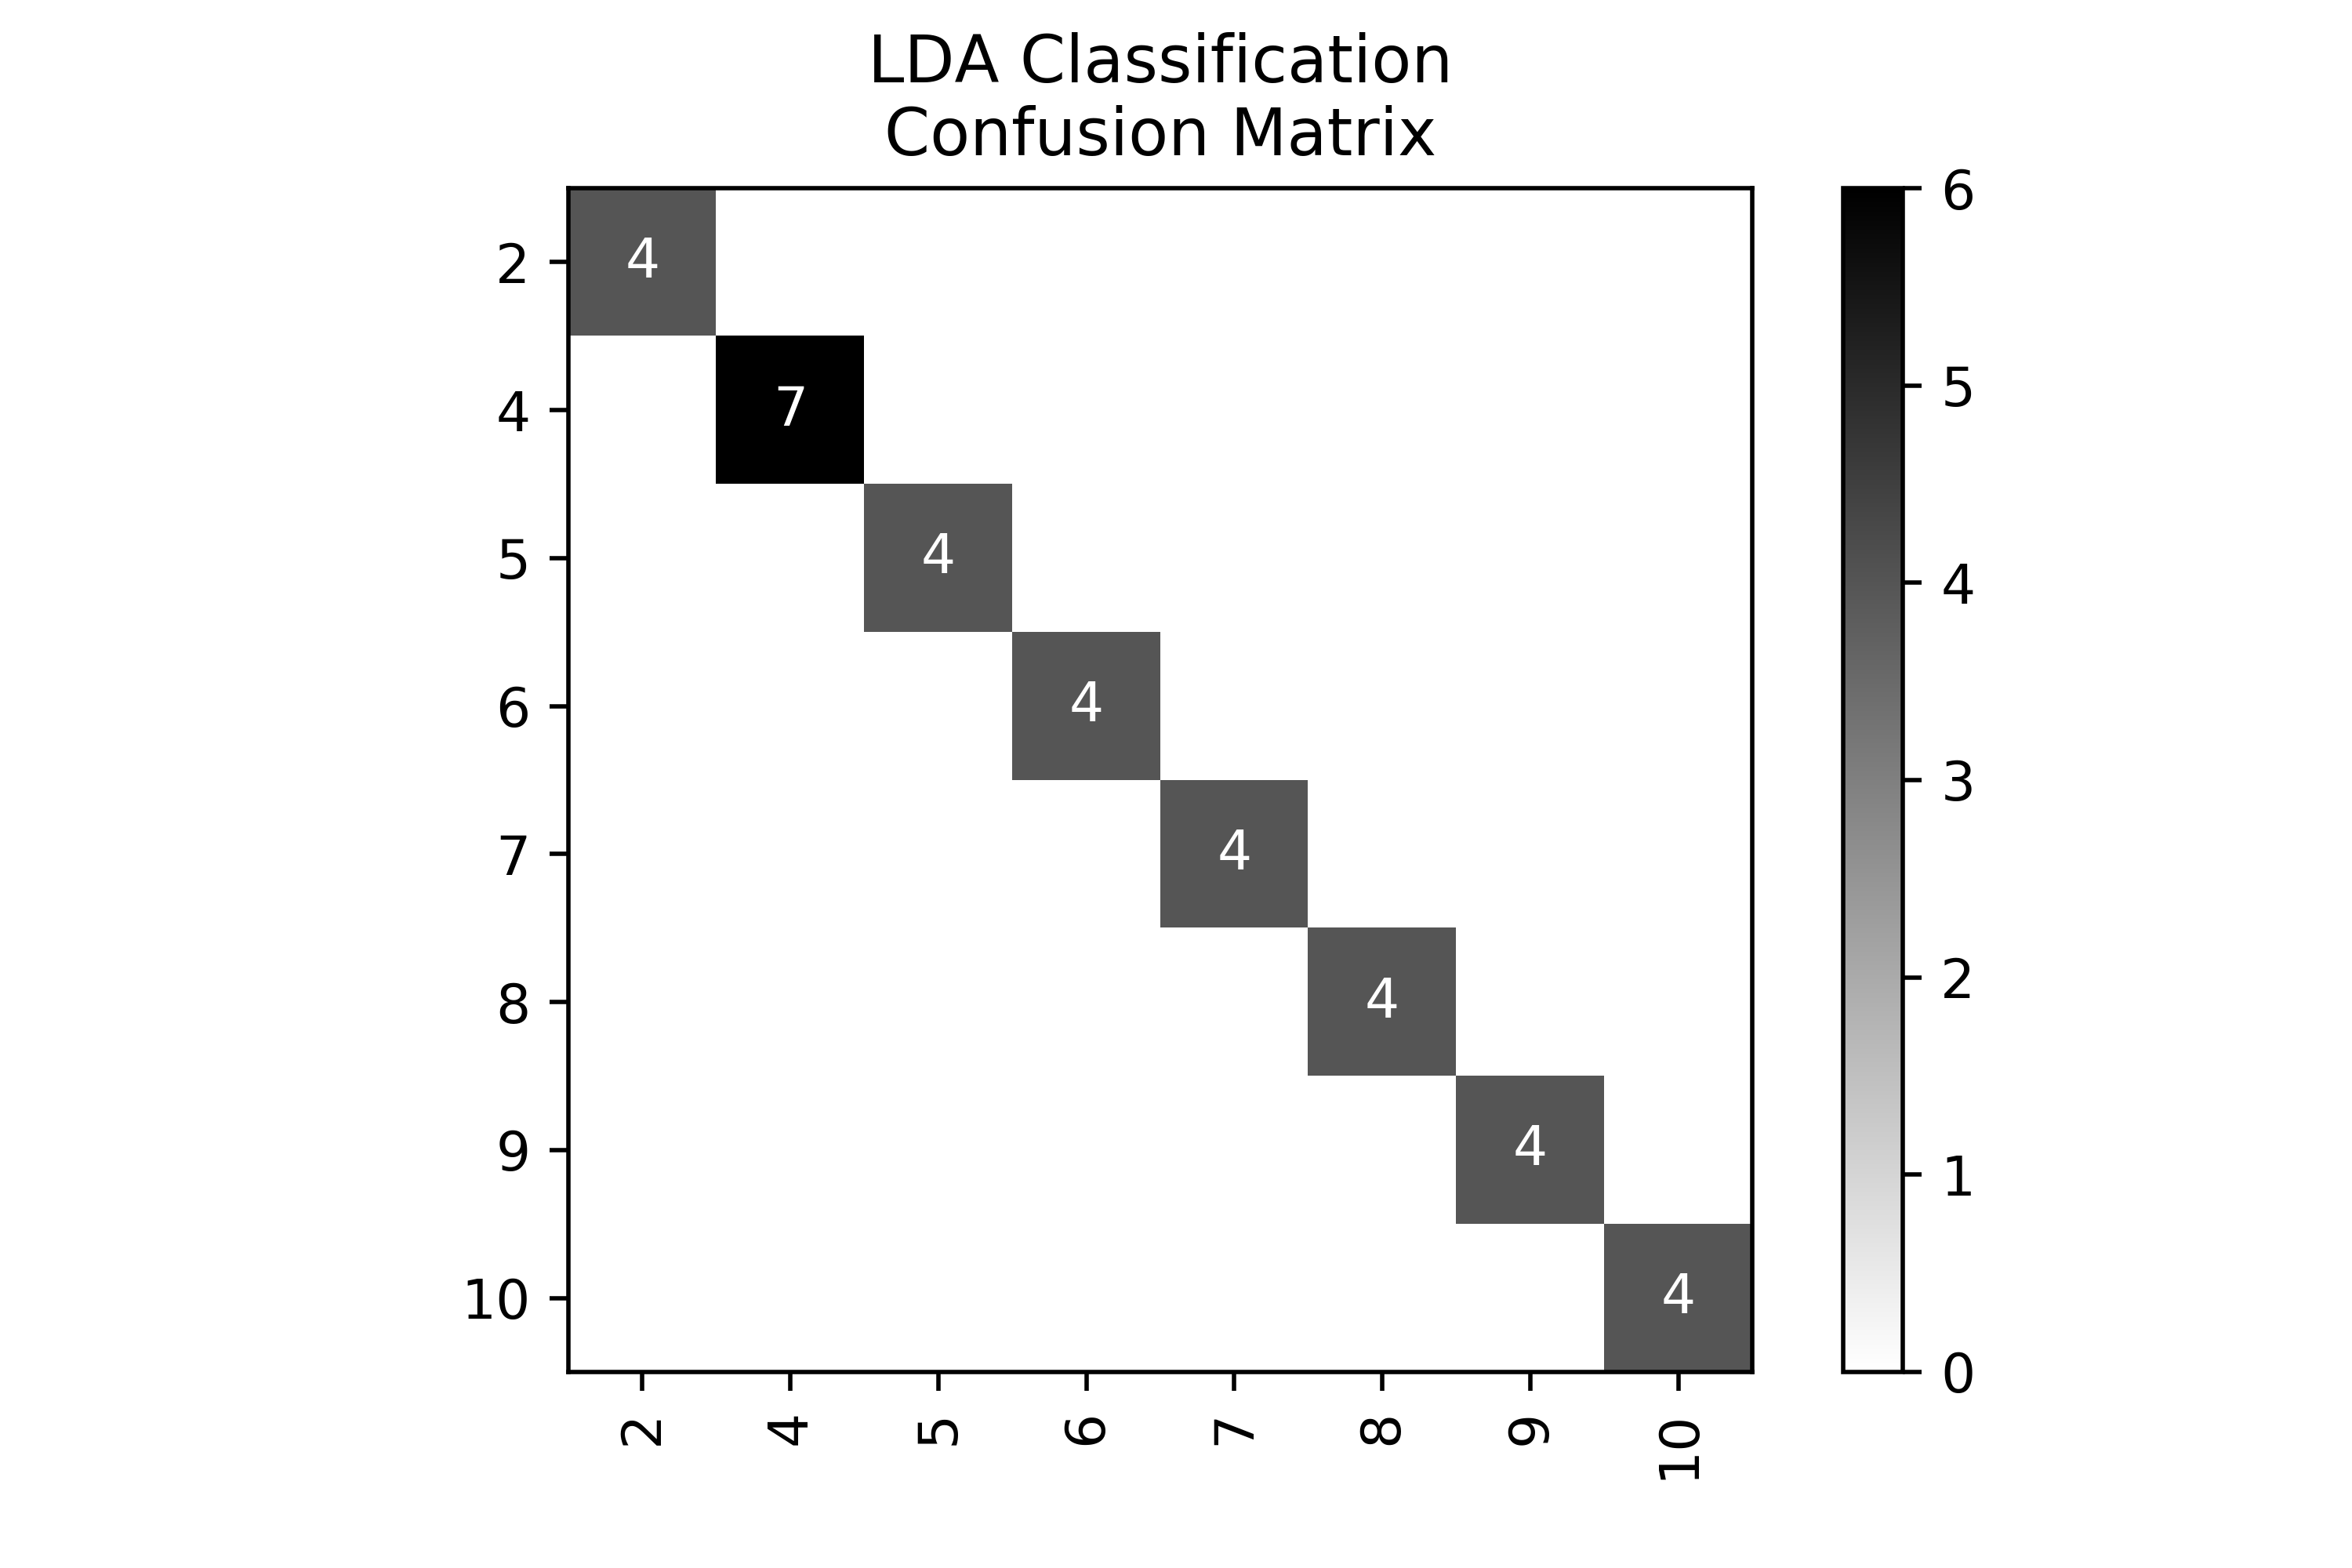
\includegraphics[height=2.5in]{LDA/LDA_classification_cfm.png}
\caption{Sample confusion matrix for one fold of three-fold cross validation for LDA model. None of the images were misclassified in this fold.}
\label{lda_confusion}
\end{figure}

A classification model using Linear Discriminant Analysis (LDA) was also tested across the four experiments. The training data was transformed using Principal Component Analysis (PCA) with the number of components varied between 1 and 12 (Fig. \ref{lda}). Using the raw color data from the first experiment, a PCA projection of the data using 12 components resulted in no loss in test accuracy ($100\%$). Concerning the second experiment, the LDA model achieved its highest accuracy of $91\%$ using 12 components. Again, the addition of color rotation to the data in the third and fourth experiments reduced the accuracy of the model to $77\%$ and $72\%$, respectively.

\begin{figure}
\centering
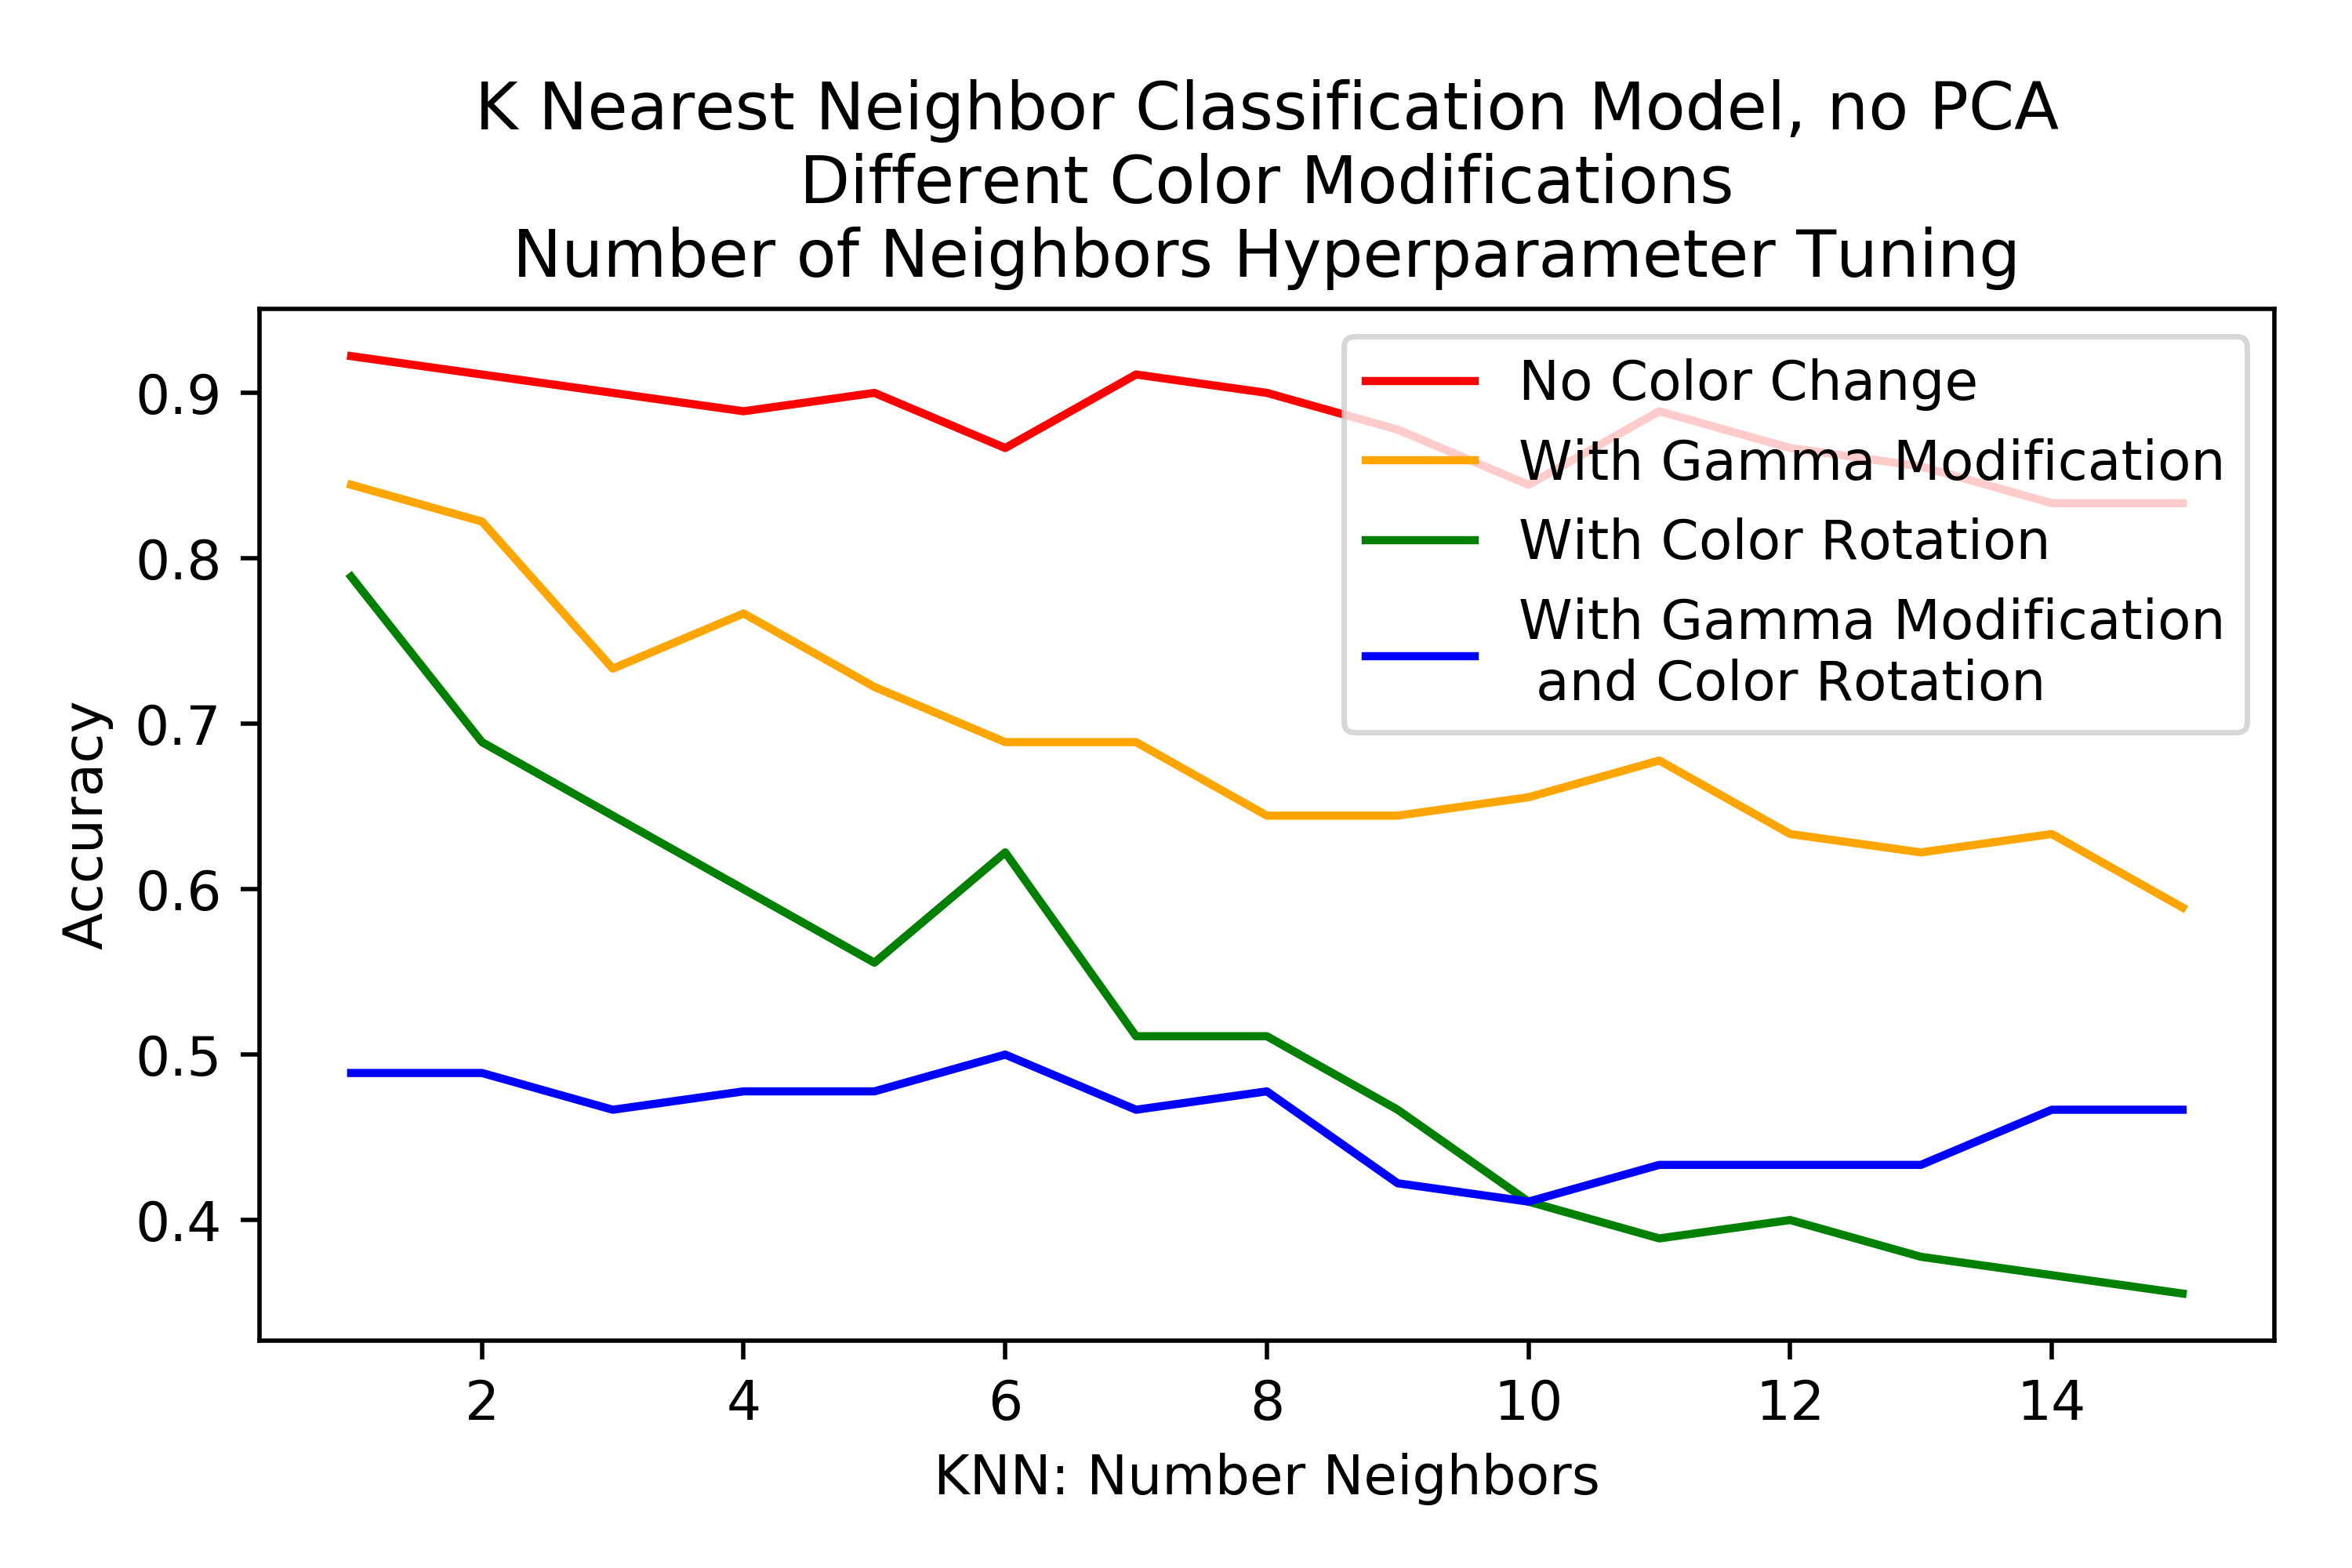
\includegraphics[height=2in]{KNN_clf_noPCA/knn_classification.png}
\caption{K Nearest Neighbor Classification Model. The Y axis is the Accuracy (percent of predicted labels that are correct) and the X axis is the number of neighbors used in the model. The four lines represent the four datasets we used: no color change, with gamma modification, with color rotation, and with both gamma modification and color rotation.}
\label{knn}

\centering
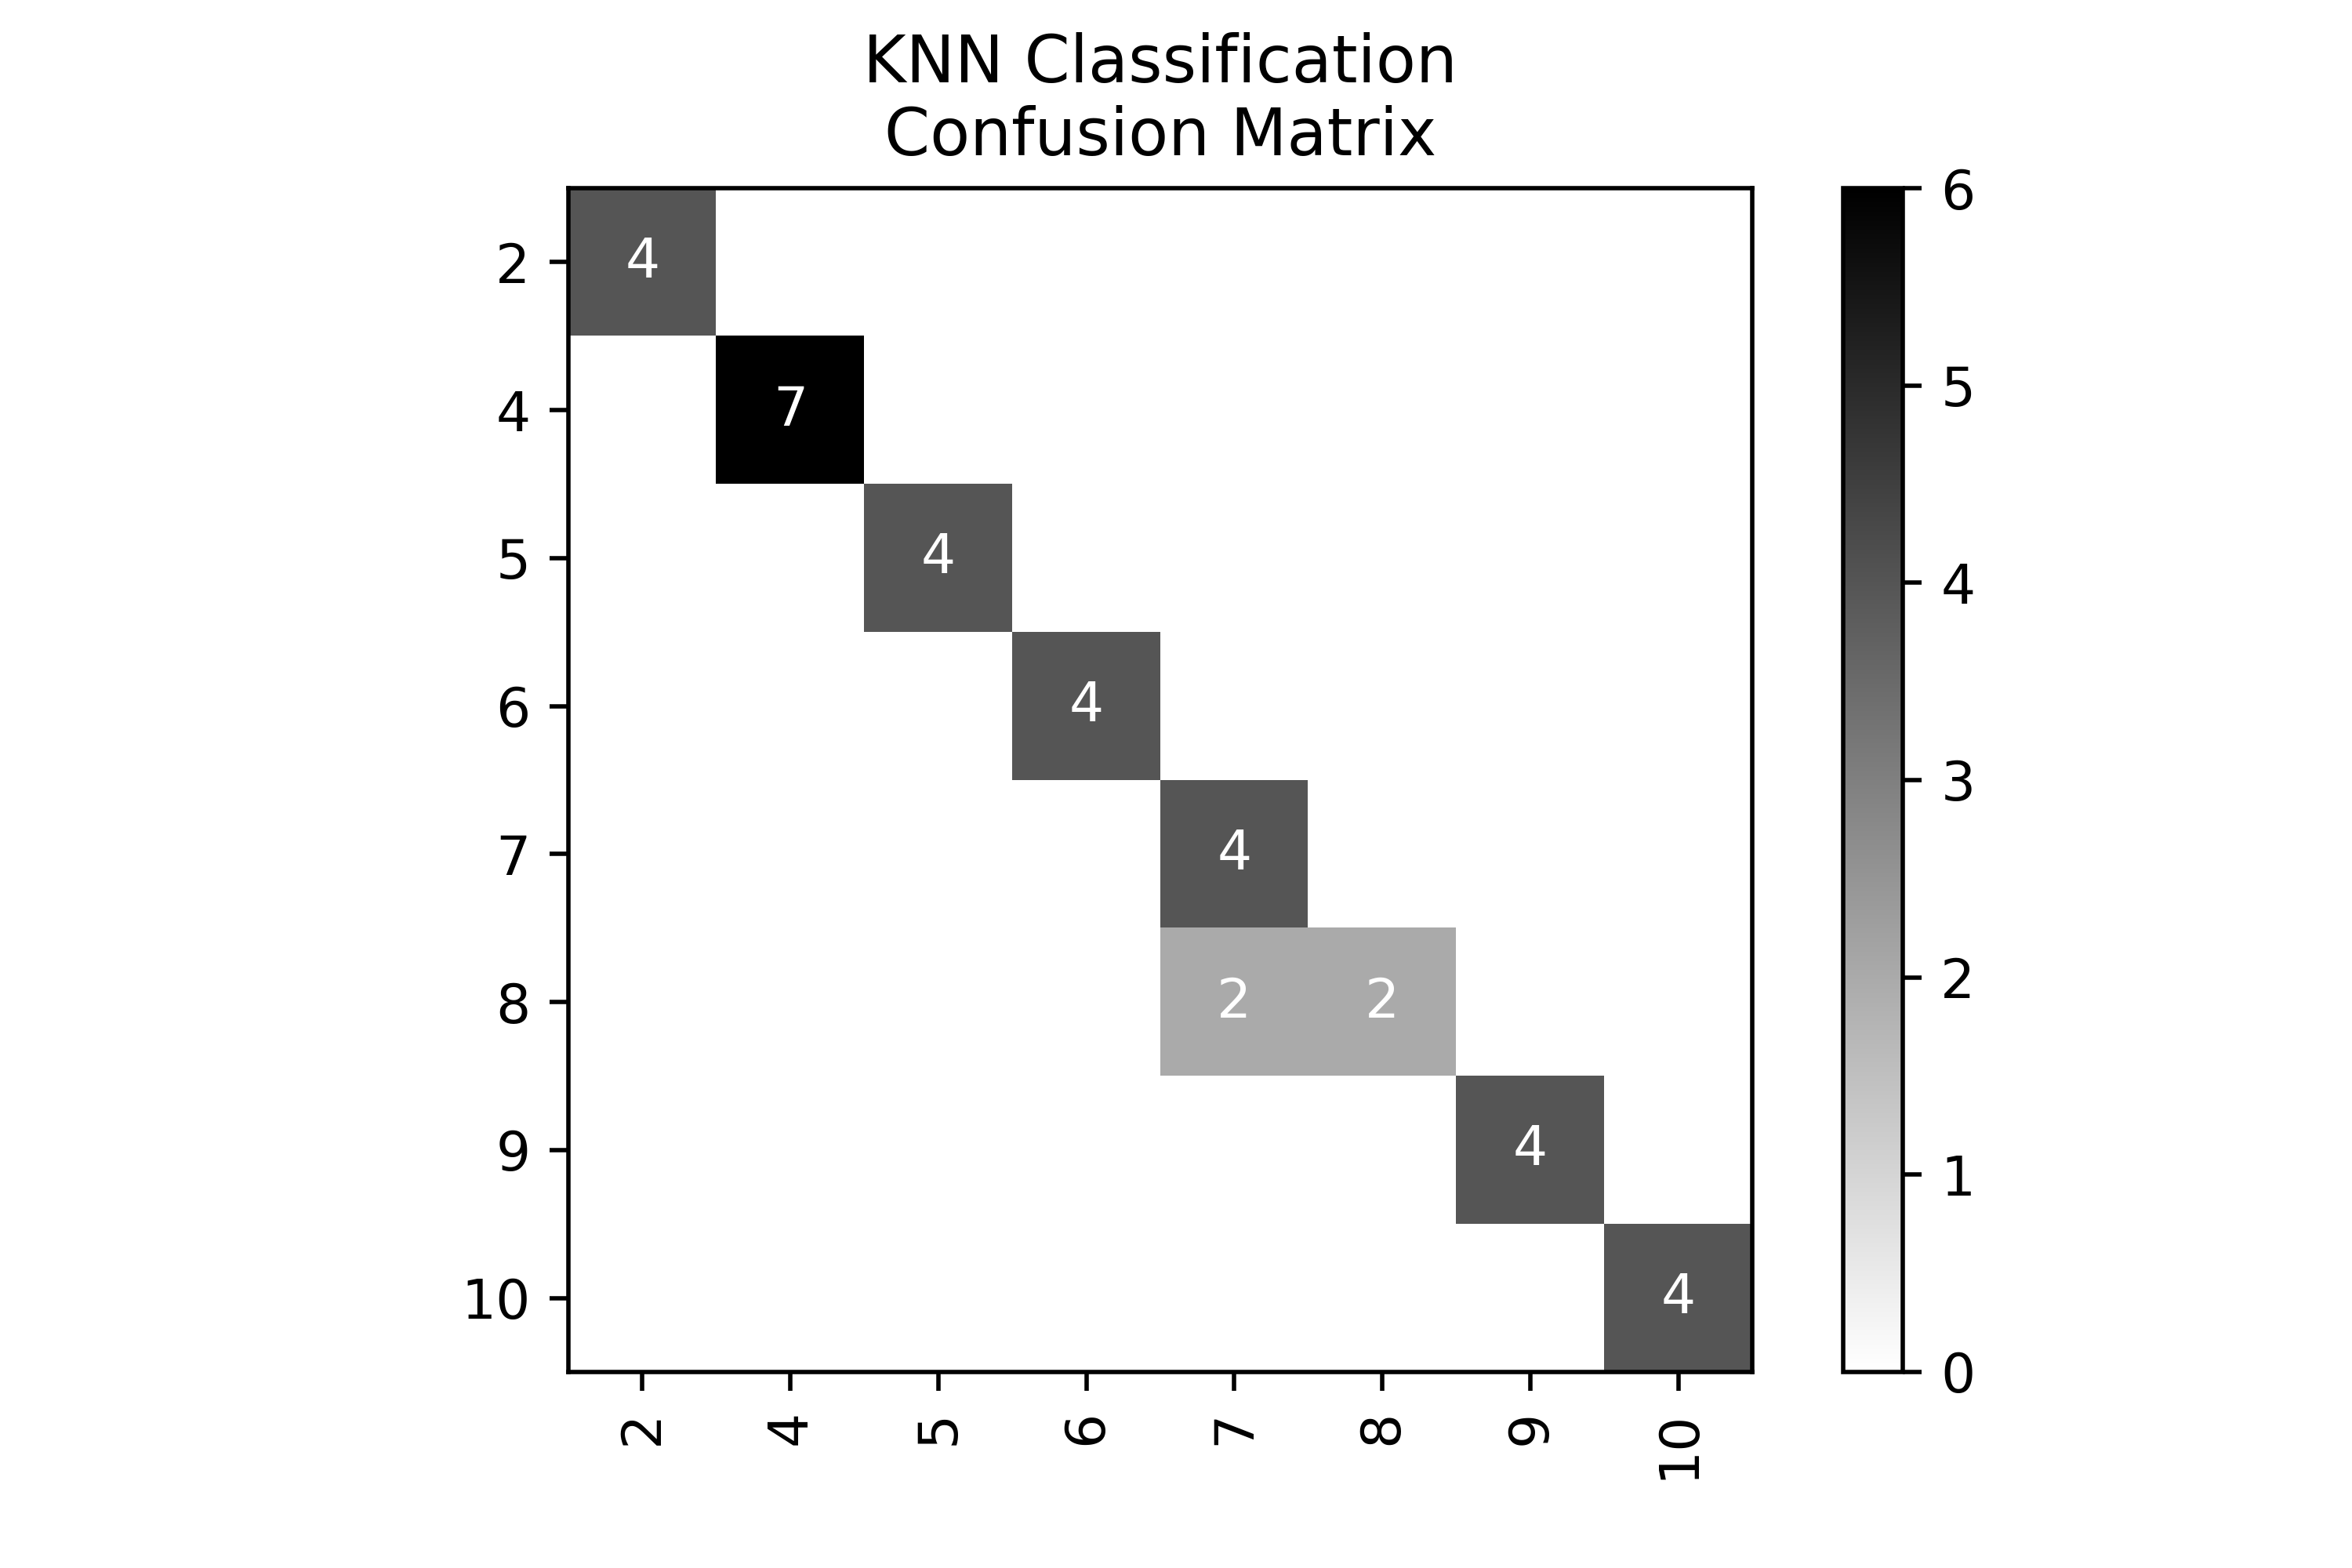
\includegraphics[height=2.5in]{KNN_clf_noPCA/KNN_classification_cfm.png}
\caption{Sample confusion matrix for one fold of three-fold cross validation for kNN model (without PCA/scaling). 2 of 35 images were misclassified.}
\label{knn_confusion}

\centering
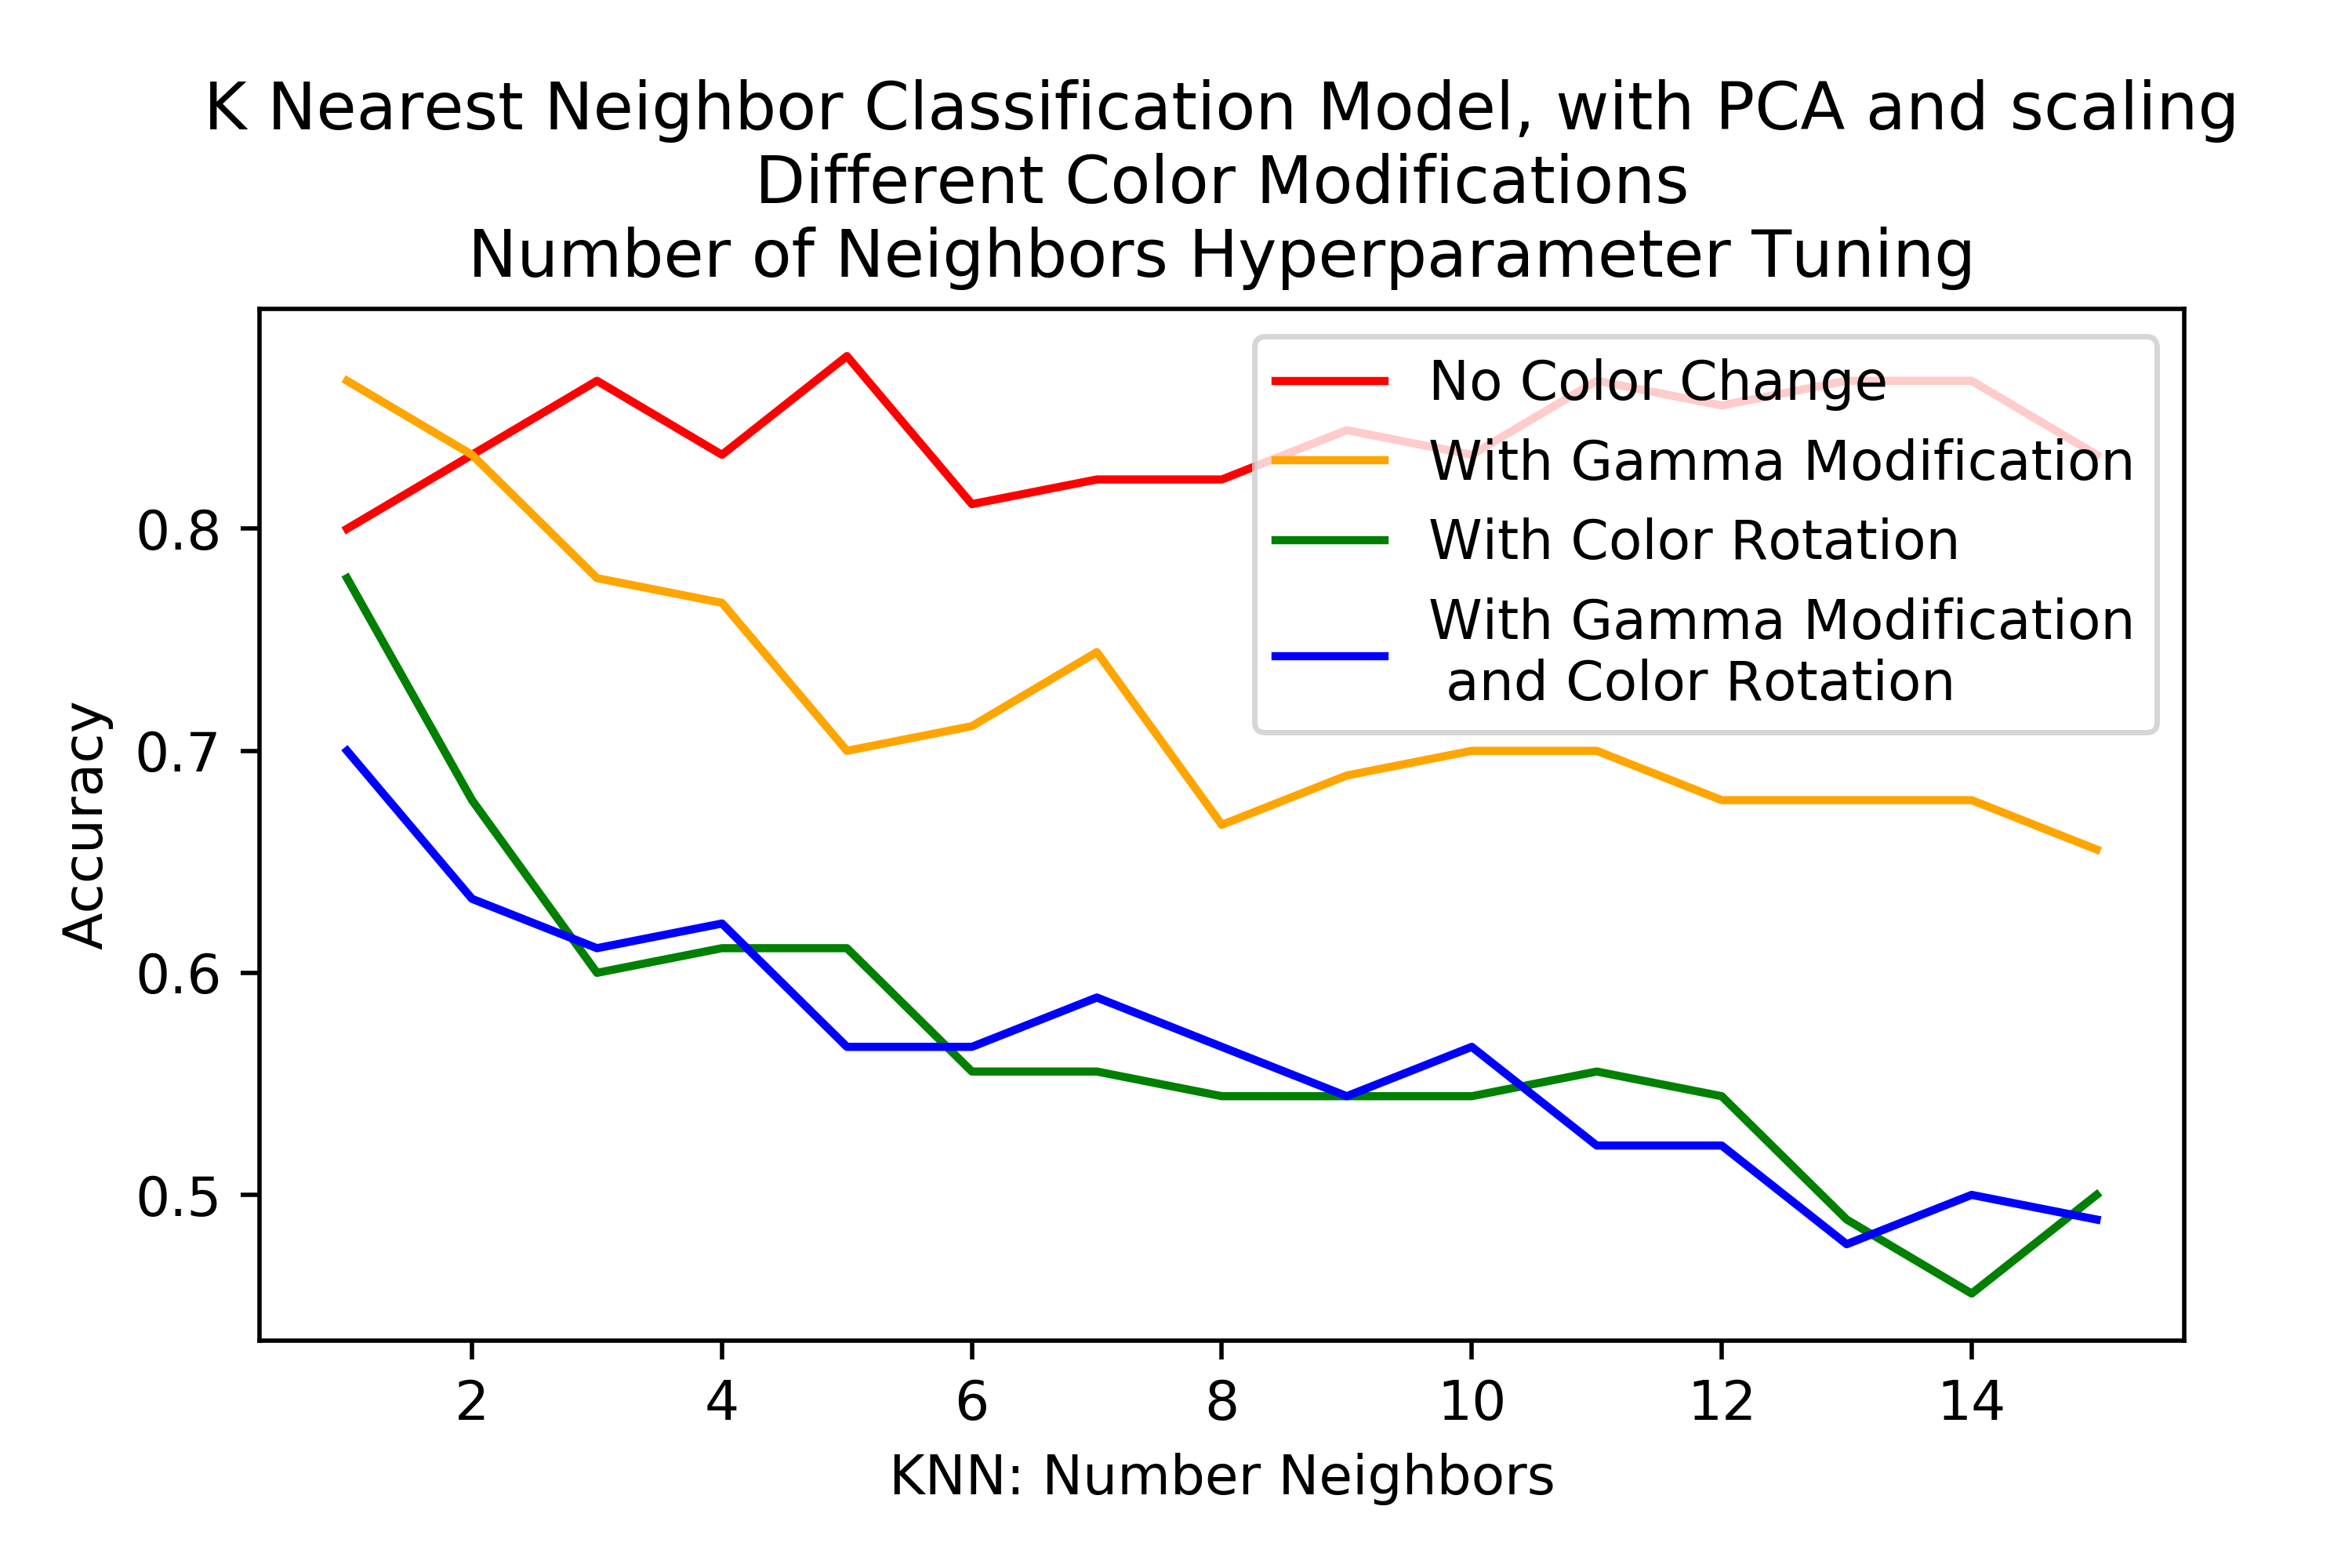
\includegraphics[height=2in]{KNN_clf_PCA/knn_classification.png}
\caption{K Nearest Neighbor Classification Model, with PCA and scaling preprocessing. The Y axis is the Accuracy (percent of predicted labels that are correct) and the X axis is the number of neighbors used in the model. The four lines represent the four datasets we used: no color change, with gamma modification, with color rotation, and with both gamma modification and color rotation.}
\label{knn_pca}
\end{figure}

Using a kNN classification model on the unscaled data across the four experiments, classification accuracies $92\%$, $84\%$, $79\%$, and $50\%$ were achieved for $k=1$, $1$, $1$, $6$, respectively (Fig. \ref{knn}, \ref{knn_confusion}). After scaling and transforming the data with PCA, classification accuracies $88\%$, $87\%$, $78\%$, and $70\%$ were achieved for $k=5$, $1$, $1$, $1$, using $2$, $3$, $8$, and $10$ PCA components, respectively (Fig. \ref{knn_pca}). Scaling and dimensionality reduction reduced accuracy on the raw color data but increased accuracy on the hue-rotated data.

\begin{figure}
\centering
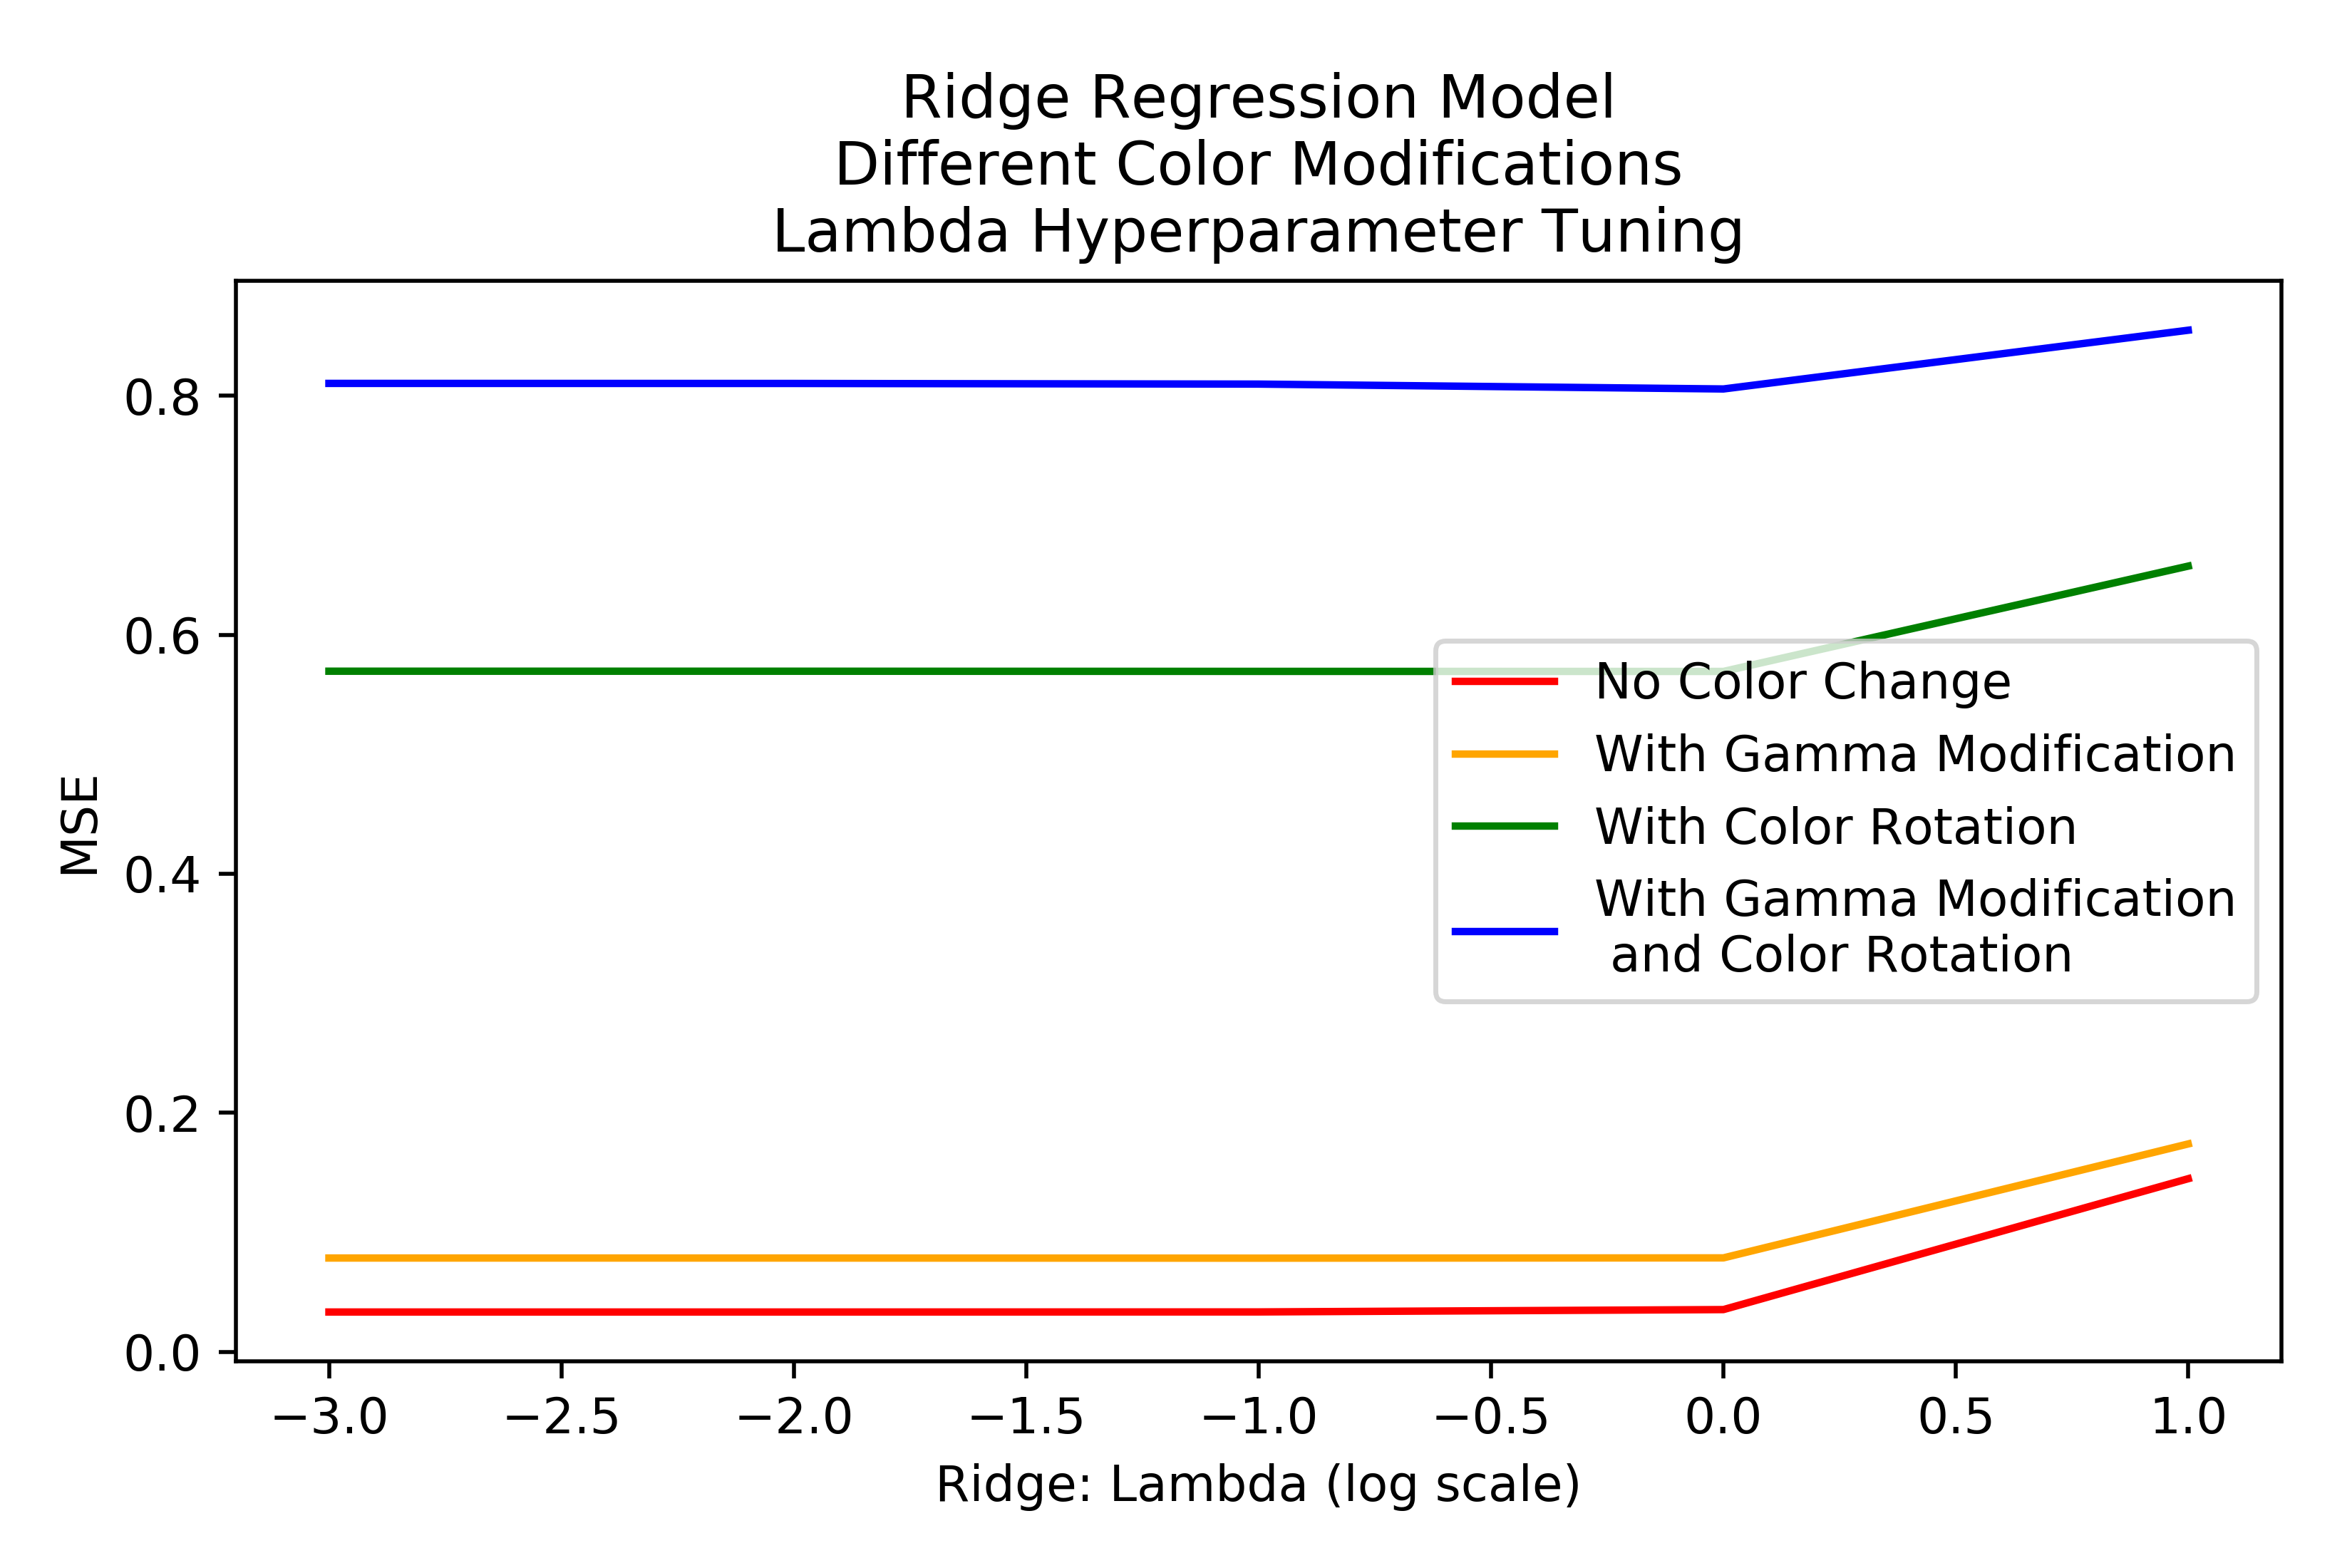
\includegraphics[height=2in]{Ridge/ridge_regression3.png}
\caption{Ridge Regression Model. The Y axis is the Mean Squared Error, which is $\frac{1}{n} \Sigma_{i=1}^n (Y_i - \hat{Y}_i)^2$ where $Y_i$ is the true value of strip $i$ and $\hat{Y}_i$ is the predicted value from our model of strip $i$, and the X axis is different levels of regularization on the model, shown on a logarithmic scale from $-3$ to $1$. The four lines represent the four datasets we used: no color change, with gamma modification, with color rotation, and with both gamma modification and color rotation.}
\label{ridge}
\end{figure}

\subsection{Regression Models}

Across the four experiments, the regression ordinary least squares models generally performed best with low ridge regularization, where $\texttt{log}_{10}(\lambda) \leq 0$  (Fig. \ref{ridge}). The lowest mean squared errors achieved across the four experiments were $0.033$, $0.078$, $0.78$, and $0.88$, respectively. The lowest mean squared error for the regression model ($0.033$) was achieved in the first experiment using the lowest regularization parameter tested ($\lambda = 0.001$). The introduction of random gamma modification slightly increased the error in the second experiment, but the color rotation added in the third and fourth experiments affected the accuracy of the model much more significantly.

\begin{figure}
\centering
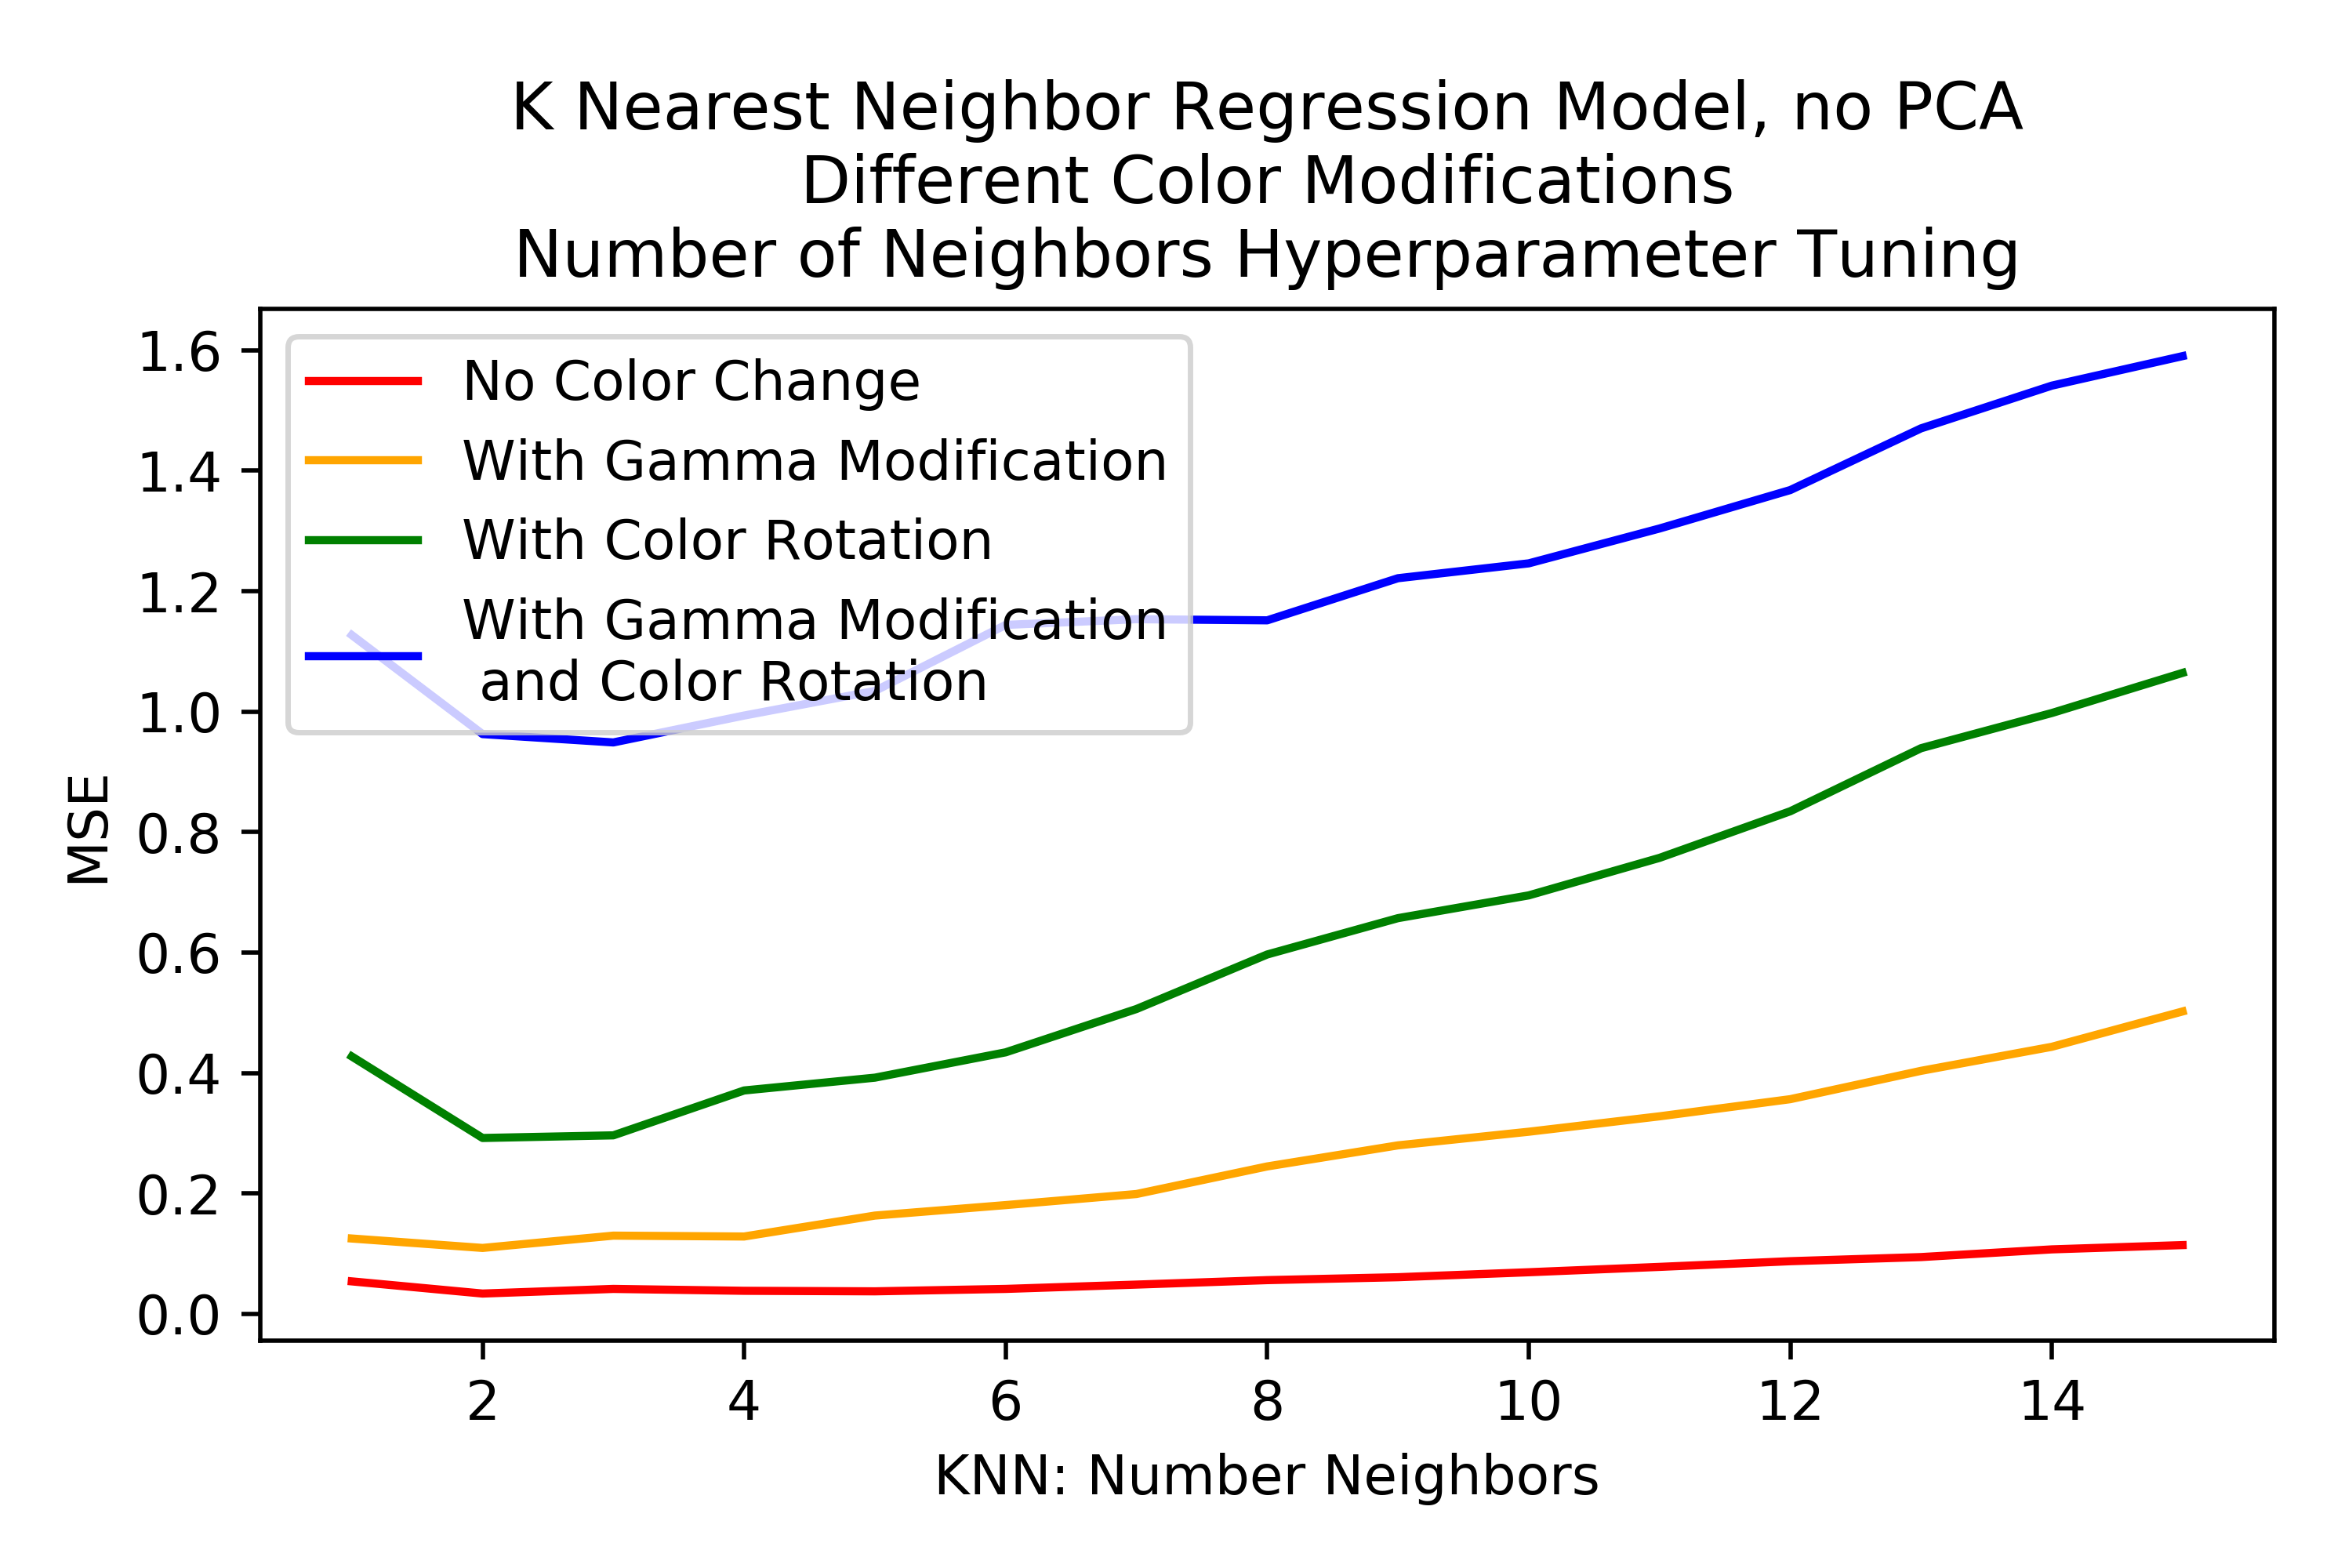
\includegraphics[height=2in]{KNN_reg_noPCA/knn_regression.png}
\caption{K Nearest Neighbor Regression Model. The Y axis is the Mean Squared Error and the X axis is the number of neighbors used in the model. The four lines represent the four datasets we used: no color change, with gamma modification, with color rotation, and with both gamma modification and color rotation.}
\label{Rknn}

\centering
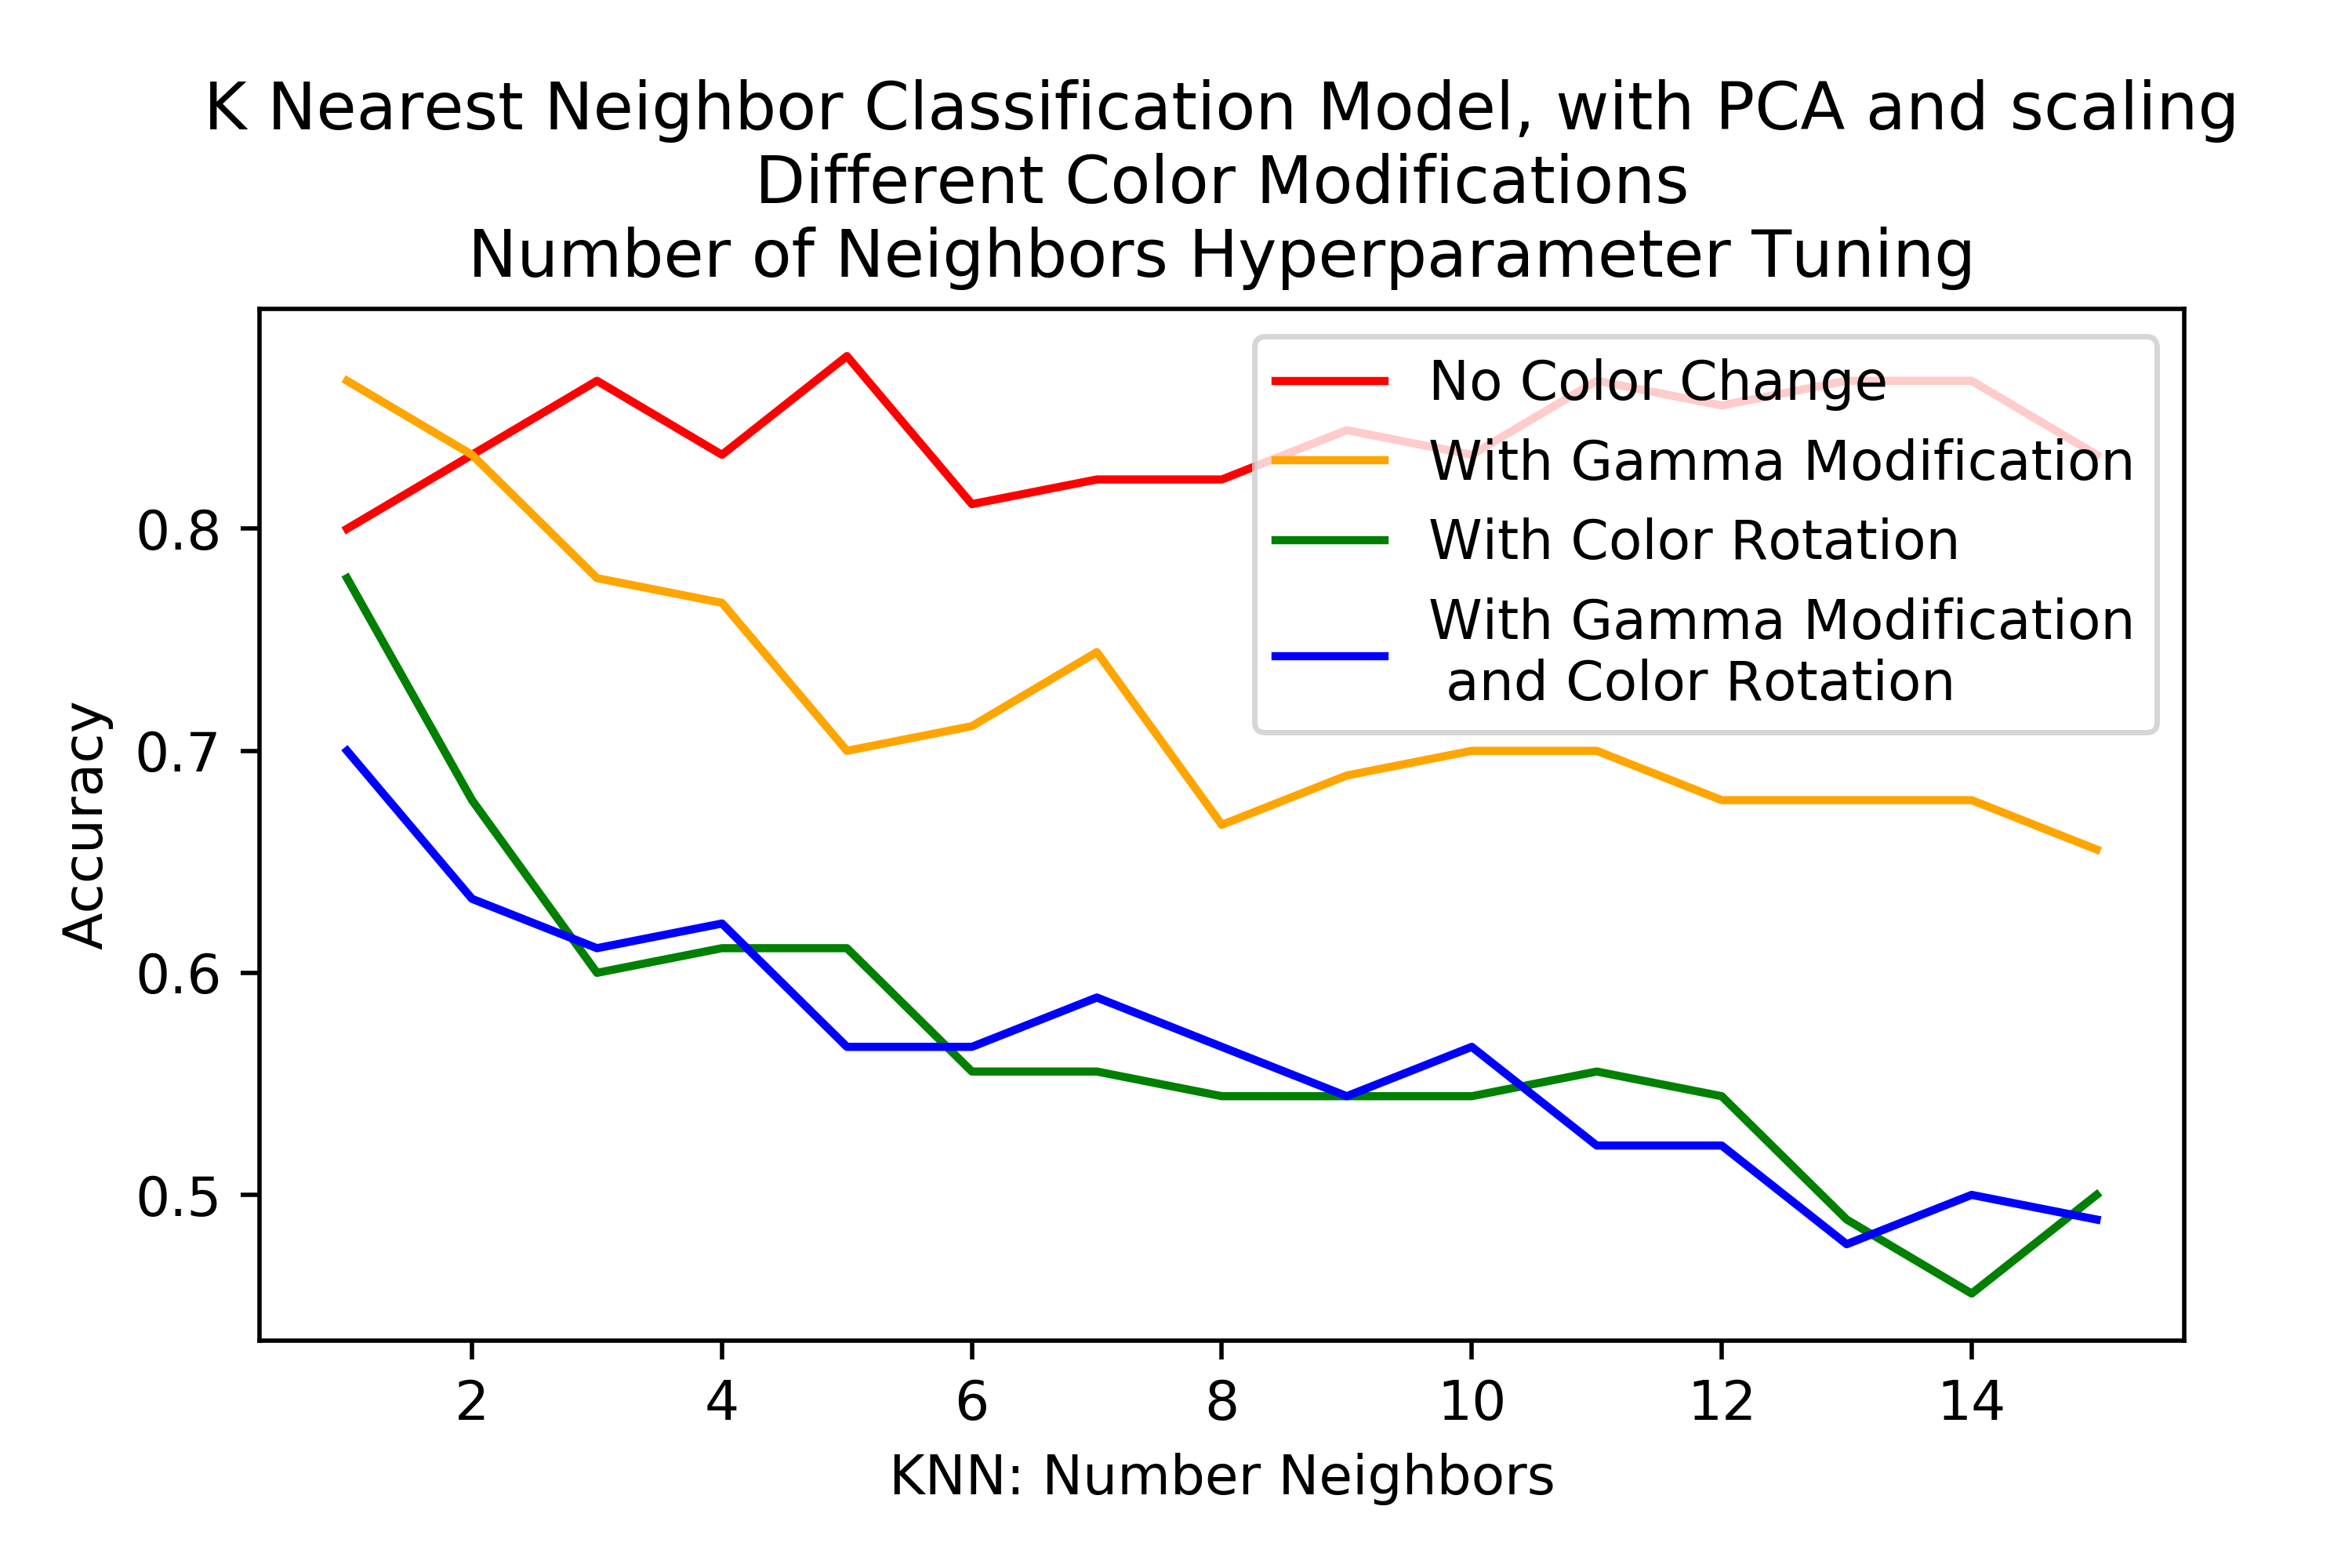
\includegraphics[height=2in]{KNN_clf_PCA/knn_classification.png}
\caption{K Nearest Neighbor Regression Model, with PCA and scaling preprocessing. The Y axis is the Mean Squared Error and the X axis is the number of neighbors used in the model. The four lines represent the four datasets we used: no color change, with gamma modification, with color rotation, and with both gamma modification and color rotation.}
\label{Rknn_pca}
\end{figure}

Using a kNN regression model on the unscaled data across the four experiments, mean squared errors of $0.034$, $0.109$, $0.292$, and $0.949$ were achieved for $k=2$, $2$, $2$, $3$, respectively (Fig. \ref{Rknn}). The lowest error on this model nearly as reliable as the lowest error achieved using ridge regression ($0.033$). After scaling and using PCA on the kNN regression model, the mean squared error for both the third and fourth experiments was greatly lowered (Fig. \ref{Rknn_pca}). For $k=2$, $2$ and $11$, $12$ PCA components, respectively, these models achieved mean squared errors of $0.197$ and $0.392$, a significant improvement over the other regression models. Concerning the first two experiments, which did not employ color rotation, kNN achieved mean squared errors of $0.046$ and $0.074$ with $k=3$, $3$ neighbors respectively.

\section{Discussion}
\subsection{Classification}
The best classification model for the unmodified color extracted data, as in our Experiment 1, was LDA with PCA pre-processing using 12 principal components. This result matched the $100\%$ accuracy that Mutlu \textquotesingle s best model, their LS-SVM, achieved. To a great extent, an LDA model is more conceptually sensible than an LS-SVM model for this application. This is because each pH value class has a single ground truth strip that corresponds to it -- all photos taken are simply noisy samples from this ground truth strip. Therefore, it makes sense that the LDA model performs so well -- it estimates the mean features of the ground truth strip and estimates a covariance matrix surrounding each mean. In other words, the mechanism of the model directly corresponds with the way data is generated. On the other hand, LS-SVM does not offer the same resemblance and in fact, the presence of outliers in a training set could significantly skew the decision boundary produced since they will incur a sizeable loss and force the hyperplane to move.

The SVM classification model also performed quite well, and outperformed the SVM model implemented by Mutlu with respect to classification accuracy. In contrast with LDA, SVM attempts to find decision boundaries by maximizing the margin between support vectors. The color rotation in Experiment 3 added significant noise, so SVM performed better on these data with lower C, or stronger regularization, to combat this noise. On the other hand, the first two experiments involving the raw color data and the data with gamma modification achieved higher accuracies as C increased, or regularization became weaker. This makes sense because the colors in this data were closer to the ground truth color values for each class. In Experiment 4, SVM was unable to achieve an accuracy greater than $80\%$. Similarly, Mutlu experienced much lower classification accuracies around $60-80\%$ when applying SVMs to data with mixed light sources.

In our experiments with discriminative classification models, we chose to use one-hot encodings as is standard for working with multiple classes; one-hot encoding ensures that there is no ordering among the classes. However, for our application, the pH value classes actually do have a natural and logical ordering (a pH value of 7 is closer to a value of 6 than 2, for example). This would be an avenue of future exploration, and we hypothesize that not using one-hot encoding may further increase our accuracy since nearby classes only differ by one or two color panels and thus, even in the presence of noisy lighting conditions, the model will have a better chance of recognizing the variations between neighboring classes as opposed to those between each pair of classes. Further, this would prevent the model from ever being in a situation in which it must decide between two classes at opposite ends of the spectrum -- with pH as a log-based scale, an incredibly inaccurate prediction like this could have disastrous implications and it would be best to avoid such a possibility.

We also experimented with projecting the extracted color data to lower-dimensional subspaces using PCA before running selected classification models. When applied to the unmodified extracted color data, we see that the different classes cluster well and are nearly separable (Fig. 3). The pH test strips used in this experiment contain four distinct panels that each react differently to separate ranges of pH values. The neat clustering found by PCA is likely due to the fact that in general, solutions with higher acidity result in brighter colors across the four panels on the pH test strip, whereas more basic solutions result in darker colors. This is why there appears to be an ordering in Figure 3, where the vertical “bars” of points for each decreasing pH class are organized from left to right. When using the PCA-projected data with the kNN (regression/classification) models, we were able to achieve lower error on the data when hue rotation was applied. This makes sense because kNN assumes that training points of the same class should be separated by smaller distances than training points between classes. This “distance” assumption tends to fall apart as the dimensionality of the data increases but this was not a concern for us since our raw color dataset already captured 12 dimensions while PCA worked to further reduce the number of dimensions. Therefore, for the hue-rotated data, PCA was able to help separate the data into clusters where kNN could be more effective with lower values of $k$. 

\subsection{Regression}
The Mutlu paper did not explore regression techniques for estimating pH, yet our experiments show that regression can be used effectively to achieve relatively small prediction error, even when the size of the training dataset is under 100 images. We chose to work with a ridge regularization model (using an L2-norm) and used cross validation to determine the optimal strength of the regularization. Since we were working with extracted color data, we chose to not use LASSO regularization (L1-norm) as there were no extraneous features to eliminate. However, had we run these experiments without image masking and color extraction techniques, LASSO regularization may be more applicable, as a regression model could be trained to ignore pixel data from the background.

The pH estimates from the best regression model tested had a very low mean squared error ($0.033$), making further research in the area of regression models for estimating pH very promising. Realistically, researchers working with pH test strips would likely prefer regression estimates for pH rather than rounded integer classification, as minute differences in pH can drastically alter the behavior of a solution. For example, in C2C12 cells, a commonly-used immortalized mouse myoblast cell line for mammalian muscular cell culture and research, the optimal growth pH is 7.0 to 7.6 \cite{product}. If we do classification, a pH of 6.6, far too low for cell survival, will be classified to 7, while a pH of 7.6, which is in the optimal growth range, will be classified to 8. While integer binning was used to achieve $100\%$ classification accuracy in the Mutlu paper, these types of models may not be as useful as regression models in practice. 

\subsection{Acknowledging Shortcomings}
While both this experiment and the Mutlu experiment used 90 pH test strips in the creation of the training dataset, both experiments should be repeated with much larger training sets for more reliable results. Given additional resources, an increased training set may have allowed for further improvements in training and test accuracy. A larger training set may have also helped both the regression and classification models become more robust with respect to noise, including lighting changes and color correction. More training data would also help reduce variance across the results of several models. 

This experiment could also be repeated with more scaling and projection techniques in order to further improve accuracy, especially concerning raw image data involving varying lighting conditions. This experiment achieved much lower errors for color rotation noise using the kNN regression models after scaling and PCA were used. 

However, as expected, the lowest mean squared errors for each model overall came from the first experiment, where neither color rotation nor gamma modification techniques were used.

Further machine learning techniques could be applied to similar datasets in order to develop more robust models. For example, neural networks could potentially extract better features from the images and perform well. However, we found that for the relatively simple dataset in this experiment, simpler models would likely achieve similar accuracies while being computationally less expensive.

\section{Conclusion}
Overall, we were able to develop both classification and regression models in this domain and obtain relatively high accuracy and low error. In spite of our similarly-sized dataset including more varied data for each pH value tested, we were able to match the classification accuracy ($100\%$) achieved by Mutlu while mimicking the various lighting changes in the data. We were also able to extend Mutlu\textquotesingle s findings using regression techniques, and successfully achieved low error in doing so.

In continuing research, a greater variety of models could be tested, and models achieving a high accuracy across varied data could potentially be exported to run on an Arduino board. This way, the process of estimating pH strips could be automated. In a similar spirit, the regression models could be integrated into a smartphone application, so that a researcher could manually take pictures of the pH strips while the models run in real time to estimate the captured pH. 

\appendices
\section*{Acknowledgment}
The authors would like to thank Professor John Christopher Anderson for supplying us with pH strips and buffer solutions.

% references section

% can use a bibliography generated by BibTeX as a .bbl file
% BibTeX documentation can be easily obtained at:
% http://mirror.ctan.org/biblio/bibtex/contrib/doc/
% The IEEEtran BibTeX style support page is at:
% http://www.michaelshell.org/tex/ieeetran/bibtex/
%\bibliographystyle{IEEEtran}
% argument is your BibTeX string definitions and bibliography database(s)
%\bibliography{IEEEabrv,../bib/paper}
%
% <OR> manually copy in the resultant .bbl file
% set second argument of \begin to the number of references
% (used to reserve space for the reference number labels box)
\begin{thebibliography}{1}
\bibitem{anderson} J. Anderson, \emph{2017\_10\_09-Final Project}, UC Berkeley, 2017.
\bibitem{mutlu} A. Mutlu, V. Kılıç, G. Özdemir, A. Bayram, N. Horzum and M. Solmaz, \emph{Smartphone-based colorimetric detection via machine learning}, The Analyst, vol. 142, no. 13, pp. 2434-2441, 2017.
\bibitem{kim} S. Kim, Y. Koo and Y. Yun, \emph{A Smartphone-Based Automatic Measurement Method for Colorimetric pH Detection Using a Color Adaptation Algorithm}, Sensors, vol. 17, no. 7, p. 1604, 2017.
\bibitem{farid} H. Farid, \emph{Blind inverse gamma correction}, IEEE Transactions on Image Processing, vol. 10, no. 10, pp. 1428-1433, 2001.
\bibitem{product} American Type Culture Collection, \emph{C2C12 (ATCC\textregistered CRL-177$^\texttt{TM}$)}, Product Sheet, Manassas, VA.

\end{thebibliography}

\end{document}
